\chapter{Reticoli e algebre di Boole}
\section{Relazioni d'ordine}

\begin{defbox}{Relazione d'ordine}\index{Relazione d'ordine}
	Sia $S$ un insieme non vuoto. Una relazione binaria $\rho$ in $S$ si dice una \textbf{relazione d'ordine largo} se è:
	\begin{enumerate}
		\item \textbf{Riflessiva}: $\forall x \in S \bigl(x \ \rho \ x \bigr)$;
		\item \textbf{Antisimmetrica}: $\forall x,y \in S \bigl((x \ \rho \ y \wedge y \ \rho \ x) \Rightarrow x = y\bigr)$;
		\item \textbf{Transitiva}: $\forall x,y,z \in S \bigl((x \ \rho \ y) \wedge (y \ \rho \ z) \Rightarrow x \ \rho \ z \bigr)$.
	\end{enumerate}
	Una relazione binaria $\rho$ in $S$ si dice una \textbf{relazione d'ordine stretto} se è :
	\begin{itemize}
		\item \textbf{Antiriflessiva:} $\forall x \in S \bigl(x \ \cancel{\rho} \ x\bigr)$.
		\item \textbf{Transitiva}
	\end{itemize}
\end{defbox}

\begin{osservation}
	Chiaramente ogni relazione di ordine stretto è necessariamente antisimmetrica. Infatti, sia $\rho$ una relazione di ordine stretto e siano $x,y \in A$ tali che $x \ \rho \ y \land y \ \rho \ x$. Per la proprietà transitiva deve essere $x \ \rho \ x $ ma per ipotesi $\rho$ è antiriflessiva. Questo vuol dire che non può essere $x \ \rho \ y \land y \ \rho \ x$ e quindi risulta vera l'implicazione $\bigl(x \ \rho \ y \land y \ \rho \ x \bigr)\implies (x=y)$ in quanto l'antecedente risulta falsa.
\end{osservation}
 Una relazione d'ordine in $S$ è in genere denotata, col simbolo $\leq$.
\begin{propbox}
	Sia $\mathbf{OL(A)}$ l'insieme di tutte le relazioni di ordine largo in $A$ e $\mathbf{OS(A)}$ l'insieme di tutte le relazioni di ordine stretto in $A$. Per ogni $\rho \in OL(A)$ è possibile definire $\rho_{\neq} \in Rel(A)$ in modo tale che, $\forall x,y \in A$:
	\begin{displaymath}
		\bigl(x \ \rho_{\neq} \ y \iff (x \ \rho \ y \land x \neq y ) \bigr) \implies \rho_{\neq} \in OS(A)
	\end{displaymath}
\end{propbox}

\begin{proof}
	Dimostriamo che la relazione $\rho_{\neq}$ gode della proprietà antiriflessiva e transitiva:
	\begin{itemize}
		\item \textbf{Antiriflessiva}: si ha che per ogni $x \in A (x \ \rho_{\neq} \ x)$ poiché $x=x$ e $x \ \rho \ x $ dato che $\rho \in OL(A)$;
		\item \textbf{Transitività}: per ogni $x,y,z \in A$ tali che $x \ \rho_{\neq} \ y \land y \ \rho_{\neq} \ z$ si ha:
		\begin{align*}
			\bigl(x \ \rho_{\neq} \ y \land y \ \rho_{\neq} \ z\bigr) &\implies (x \ \rho \ y \land x \neq y) \land (y \ \rho \ z \land y \neq z) & \text{\textcolor{gray}{Per ipotesi}}\\
			&\implies x \ \rho \ z \land x \neq z & \text{\textcolor{gray}{Sfruttando la transitività di $\rho$}}
		\end{align*}
	\end{itemize}
\end{proof}

\begin{propbox}
	Per ogni $\sigma \in OS(A)$ è possibile definire $\sigma_{=} \in Rel(A)$ in modo tale che, per ogni $x,y \in A$:
	\begin{displaymath}
		\bigl( x \ \sigma_{=} \ y \iff (x \ \sigma \ y \lor x = y ) \bigr) \implies \sigma_{=} \in OL(A)
	\end{displaymath}
\end{propbox}

\begin{proof}
	Dimostriamo che $\rho_{=}$ è riflessiva, antisimmetrica e transitiva:
	\begin{itemize}
		\item \textbf{Riflessiva:} per ogni $x \in A$ si ha $x \ \rho_{=} \ x $ poiché $x=x$;
		\item \textbf{Antisimmetria:} negando la proprietà devono esistere $x,y \in A$ per i quali $\bigl(x \ \sigma_{=} \ y \land y \ \sigma_{=} \ x \land x \neq y \bigr)$ il che sarebbe equivalente a dire che $\bigl( (x \ \sigma \ y \lor x = y) \land (y \ \sigma \ x \lor y=x) \land (x \neq y) \bigr)$, ovvero $(x \ sigma \ y) \land (y \ \sigma \ x) \land (x \neq y)$ il che è assurdo in quanto $\sigma$ è antisimmetrica. Quindi $\sigma_{=}$ è antisimmetrica.
		\item \textbf{Transitività:} per ogni $x,y,z \in A$ tali che $x \ \sigma \ y $ e $y \ \sigma \ z$ si ha:
		\begin{displaymath}
			x \ \sigma \ y \land y \ \sigma \ z \implies (x \ \sigma \ y \lor x = y) \land (y \ \sigma \ z \lor y=z) \\
		\end{displaymath}
		Nel caso in cui $x=y \land y = z$ si ha $x=z$, ovvero $x \ \sigma_{=} \ z$. Altrimenti, da $x \ \sigma \ y \land y \ \sigma \ z$ segue $x \ \sigma \ z$ e, per la transitività di $\sigma$ si ottiene $x \ \sigma_{=} \ z$.
	\end{itemize}
\end{proof}

\begin{propbox}
	Le applicazioni $\rho \in OL(A) \mapsto \rho_{=} \in OS(A)$ e $\sigma \in OS(A) \mapsto \sigma_{=} \in OL(A)$ sono biettive e l'una l'inversa dell'altra.
\end{propbox}

\begin{proof}
	Sia $\overline{\rho}$ la relazione duale di $\rho$ e sia $(\overline{\rho})^{\#}$ il suo grafico. Definiamo:
	\begin{enumerate}
		\item $\rho$ antiriflessiva se e soltanto se: $\Delta_{A} \cap \rho^{\#} = \emptyset$;
		\item $\rho$ antisimmetrica se e soltanto se: $\rho^{\#} \cap (\overline{\rho})^{\#} \subseteq \Delta_{A}$;
	\end{enumerate}
	Inoltre, si ha $(\rho_{\neq})^{\#} = \rho^{\#} \setminus \Delta_{A}$ e $(\sigma_{=})^{\#} = \sigma^{\#} \cup \Delta_{A}$. Allora il grafico di $(\rho_{\neq})_{=}$ risulta:
	\begin{align*}
		\bigl((\rho_{\neq})_{=}\bigr)^{\#} = \bigl(\rho^{\#} \setminus \Delta_{A}\bigr) \cup \Delta_{A}= \rho^{\#}
	\end{align*}
	dualmente per $(\sigma_{=})_{\neq}$
\end{proof}

\marker{yellow!40}{yellow!20!black}{
	La relazione identica $\iota_{S}$ è una relazione d'ordine in $S$, ed è chiaro che $\iota_{S}$ \textbf{è l'unica relazione di equivalenza in $S$ che sia anche una relazione d'ordine}.
}


\begin{osservation}
	Qualunque sia l'insieme $S$, la relazione binaria $\rho$ in $\mathcal{P}(S)$, definita ponendo:
	\begin{displaymath}
		x \ \rho \ y \Leftrightarrow x,y \in \mathcal{P}(S) \wedge x \subseteq y
	\end{displaymath}
	è una relazione d'ordine in $\mathcal{P}(S)$ chiamata \textbf{relazione di inclusione} e denotata con il simbolo $\subseteq$.
\end{osservation}


\begin{example}
	Un esempio di relazione d'ordine stretto è fornito dalla relazione binaria $\rho$, definita nell'insieme $\mathcal{P}(S)$ delle parti di un insieme $S$ ponendo:
	\begin{displaymath}
		x \ \rho \ y \Leftrightarrow x \subset y
	\end{displaymath}
	cioè se e soltanto se:
	\begin{displaymath}
		x \subseteq y \wedge x \neq y
	\end{displaymath}
	Tale relazione viene denotata col simbolo $\subset$.
\end{example}

\begin{example}\label{exmp:divisibilità}
	Sia $(\mathbb{N}, \cdot)$ un monoide abeliano. La relazione di divisibilità $\divides$ in $(\mathbb{N},\cdot)$ indicata da $\divides$ oppure da $\divides_{(\mathbb{N},\cdot)}$ è definita dalla formula:
	\begin{equation}
		\forall a,b \in S \bigl( a \divides b \iff \exists c \in \mathbb{N} (b = ac)\bigr)
	\end{equation}
	è una relazione di ordine parziale:
	\begin{enumerate}
		\item Per ogni $a \in \mathbb{N} \bigl( a \divides a \bigr)$, infatti $a = a \cdot 1$.
		\item Per ogni scelta di $a,b \in \mathbb{N}$, se $a \divides b$ e $b \divides a$, allora $a = b$: infatti esistono $q,q' \in \mathbb{N}$ tali che $b=a \cdot q$, $a=b \cdot q'$, quindi $a= a \cdot q \cdot q'$ e $a \cdot (1-q \cdot q') = 0$; se $a \neq 0$ deve essere $1-q \cdot q' = 0$, per cui $q = q' = 1$ e $a=b$; se invece $a=0$, anche $b=0$ e dunque nuovamente $a=b$;
		\item Per ogni scelta di $a,b,c \in \mathbb{N}$, se $a \divides b$ e $b \divides c$, allora $a \divides c$. Infatti, siano $q$ e $q' \in \mathbb{N}$ tali che $b= a \cdot q$ e $c = b \cdot q'$ allora $c = a \cdot (q \cdot q')$.
	\end{enumerate}
Altri risultati importanti sulla relazione di divisibilità saranno mostrati nella sezione \ref{sez:associati}.
\end{example}

\subsection{Insiemi ordinati}\label{sez:ordine}
\begin{defbox}{Insieme ordinato}
	Sia $S$ un insieme non vuoto e sia $\leq$ una relazione d'ordine in $S$. La coppia $(S, \leq)$ si chiama \textbf{insieme ordinato} (parzialmente), e l'insieme $S$ si dice \textbf{sostegno} di tale insieme ordinato.
	
\end{defbox}

\begin{example}
Sono insiemi ordinati:
		\begin{displaymath}
			\begin{array}{llll}
				(\mathbb{R},\leq) & (\mathbb{Q},\leq) & (\mathbb{Z}, \leq) & (\mathbb{N}, \leq)
			\end{array}
		\end{displaymath}
		dove $\leq$ è l'ordine usuale (ad esempio definito su $\mathbb{R}$ da $x \leq y$ se $y-x\geq0$, ovvero se esiste $a \in \mathbb{R}$ tale che $y-x=a^{2}$).
\end{example}

\begin{defbox}{Relazione d'ordine totale}
	Se $(S,\leq)$ è un insieme ordinato, gli elementi $x$ e $y$ di $S$ si dicono \textbf{confrontabili} se risulta $x \leq y$ oppure $y \leq x$, cioè se il grafico di $\leq$ contiene almeno una delle coppie $(x,y)$ e $(y,x)$. Se due qualunque elementi di $S$ sono confrontabili allora la relazione $\leq$ si dice una \textbf{relazione d'ordine totale} e la coppia $(S,\leq)$ è un \textbf{insieme totalmente ordinato}.
\end{defbox}

\begin{example}
\begin{enumerate}
		\item $(\mathcal{P}(X), \subseteq)$ non è un insieme totalmente ordinato se $X$ ha più di due elementi. Infatti, se $a_{1}, a_{2}$ sono elementi distinti di $X$, allora $\{a_{1}\}, \{a_{2}\} \in \mathcal{P}(X)$ e $\{a_{1}\} \nsubseteq \{a_{2}\}, \{a_{2}\}\nsubseteq \{a_{1}\}$. In questo caso diremo che $(\mathcal{P}(X),\subseteq)$ è un insieme \textbf{parzialmente ordinato}.
		\item L'insieme ordinato $(\mathbb{N}, \divides)$ non è totalmente ordinato. Basta considerare gli elementi 2 e 3 per vedere che $2 \ndivides 3$ e $3 \ndivides 2$.
		\item Gli insiemi $(\mathbb{R},\leq)$, $(\mathbb{Q},\leq)$, $(\mathbb{Z},\leq)$, dove $\leq$ è l'ordine usuale, sono totalmente ordinato.
\end{enumerate}
\end{example}

\begin{defbox}{Funzioni crescenti}
	Se $(S, \rho)$ e $(T,\sigma)$ sono insiemi ordinati, un'applicazione $f: S \rightarrow T$ si dice \textbf{crescente} se e soltanto se:
	\begin{equation}
		\forall a,b \in S \bigl(a \ \rho \ b \implies f(a) \ \sigma \ f(b) \bigr)
	\end{equation}
\end{defbox}

\begin{teorbox}[Isomorfismi tra insiemi ordinati]\label{thm:iso_ordinati}
	Siano $(S,\leq_{S})$ e $(T, \leq_{T})$ due insiemi ordinati. Si dice che $f: S \rightarrow T$ è un isomorfismo\footnote{Detto anche \textbf{isomorfismo d'ordine}} tra le strutture $(S,\leq_{S})$ e $(T,\leq_{T})$ se e soltanto se:
	\begin{enumerate}
		\item $f$ è biettiva;
		\item $f$ è crescente da $(S,\leq_{S})$ a $(T, \leq_{T})$: $\forall x,y \in S \bigl(x \leq_{S} y \implies f(x) \leq_{T} f(y) \bigr)$;
		\item $f^{-1}$ è crescente da $(T, \leq_{T})$ a $(S,\leq_{S})$: $\forall x,y \in T \bigl( x \leq_{T} y \implies f^{-1}(x) \leq_{S} f^{-1}(y) \bigr)$.
	\end{enumerate}
\end{teorbox}

\subsection{Minimo, massimo, minimali e massimali}
\begin{defbox}{Minimo e massimo di un insieme}
	Sia $(S,\leq)$ un insieme ordinato, e sia $X$ una parte non vuota di $S$. Un elemento $\bar{x}$ di $X$ si dice \textbf{minimo} di $X$ se risulta:
	\begin{displaymath}
		\forall x \in X \bigl( \bar{x} \leq x \bigr)
	\end{displaymath}
	L'eventuale minimo della parte non vuota $X$ di $S$ si denota col simbolo $min \ X$. Un elemento $\bar{\bar{x}} \in X$ si dice invece \textbf{massimo} se risulta:
	\begin{displaymath}
		\forall x \in X \bigl(x \leq \bar{\bar{x}}\bigr)
	\end{displaymath}
	L'eventuale massimo di $X$ si denota col simbolo $max \ X$.
	
\end{defbox}

\begin{defbox}{Elementi minimali e massimali}
	Sia $(S,\leq)$ un insieme ordinato. Un elemento $x$ di $S$ si dice \textbf{minimale} se non esiste alcun elemento $y$ di $S$ tale che $y < x$. Si dice invece che $x$ è un elemento \textbf{massimale} di $S$ se non esiste alcun elemento $y \in S$ tale che $x < y$.
\end{defbox}

Dalle definizioni segue, in particolare, che ogni elemento massimo (minimo) è anche un elemento massimale (minimale).  Non sempre, però, vale il contrario. Osserviamo anche che un insieme ordinato può avere diversi elementi minimali (o massimali). 

\begin{example}
	\begin{enumerate}
		\item Qualunque sia l'insieme $S$, nell'insieme ordinato $(\mathcal{P}(S), \subseteq)$ si ha:
		\begin{displaymath}
			\begin{array}{c}
				min \ \mathcal{P}(S) = \varnothing \\
				max \ \mathcal{P}(S) = S
			\end{array}
		\end{displaymath}
		
		\item L'insieme ordinato $(\mathbb{N}, \divides)$ ha minimo $1$, infatti $1 \divides n$ per ogni $n \in \mathbb{N}$, e massimo $0$, infatti $n \divides 0$ per ogni $n \in \mathbb{N}$. Se però togliamo $0$ e consideriamo $\mathbb{N}^{*}= \mathbb{N}\setminus\{0\}$, l'insieme ordinato $(\mathbb{N}^{*}, \divides)$ non ha massimo.
		\item Nell’insieme ordinato $ (\mathbb{N}\setminus \{1\}, \divides)$ dei numeri naturali diversi da 1 ordinato per divisibilità, gli elementi minimali sono tutti i numeri primi (positivi).
		\item Consideriamo, per un $n \in \mathbb{N}$, l'insieme $Div(n)=\{a \in \mathbb{N} \; | \; a \divides n\}$ dei divisori di $n$. Chiaramente in $(Div(n),\divides)$ si ha $min(Div(n))=1$ e $max(Div(n))=n$.
		
		\item Consideriamo l'insieme $\{1,2,3\}$ ordinato dalla divisibilità. Così:
	\begin{displaymath}
		1 \divides 2, \qquad 1 \divides 3, \qquad 2 \ndivides 3, \qquad 3 \ndivides 2
	\end{displaymath}
		Quindi 1 è minimo (minimale), mentre 2, 3 sono massimali, ma non massimi.
		\item Sia $Z=\{1,2,3\}$ e sia $X = \{A \in \mathcal{P}(Z) \; | \; |A| \text{ è pari}\}$. Allora $\emptyset = min(X)$, e dunque è l'unico elemento minimale di $X$, mentre $\{1,2\}$, $\{1,3\}$, $\{2,3\}$ sono elementi massimali di $(X,\subseteq)$.
	\end{enumerate}
\end{example}

\begin{propbox}
	Se $x \in (S,\leq)$ è il minimo allora $x$ è l'unico minimale. (Rispettivamente con il massimo).
\end{propbox}

\begin{proof}
	Supponiamo esista un elemento $y'$ minimale in $(S,\leq)$ allora deve valere:
	\begin{align*}
		(y' \ \text{minimale in $S$}) \implies  (y' \leq x)
	\end{align*}
	Sappiamo però che $x$ è il minimo in $(S,\leq)$, quindi per ogni elemento $y \in S$ vale sicuramente  $(x \leq y)$. Allora, mettendo insieme le due proprietà varrebbero contemporaneamente:
	\begin{align*}
		\bigl((x \leq y') \land (y' \leq x) \bigr) \implies x=y'
	\end{align*}
\end{proof}

Il minimo ed il massimo di un insieme, se esistono sono unici. In un insieme totalmente ordinato, \textit{il concetto di minimo e minimale coincidono}. Analogamente con massimo e massimale.


\begin{teorbox}
	Sia $(S,\rho)$ un insieme ordinato finito non vuoto. Allora $(S,\leq )$ ha elementi minimali ed elementi massimali.
\end{teorbox}

\begin{proof}
	Supponiamo che $(S,\leq )$ non abbia minimali. Poiché $S \neq \varnothing$ allora esiste un elemento $x_{0} \in S$. Fissato tale elemento, sicuramente questo non sarà un elemento minimale  (in quanto abbiamo assunto che non sono presenti in $S$), allora esiste un elemento $x_{1} \in S$ tale che $x_{1} < x_{0}$ con $x_{1}$ non minimale. Allora possiamo considerare un ulteriore elemento $x_{2} \in S$ e $x_{2} < x_{1} < x_{0}$. Proseguendo in questo modo è possibile definire una successione $(x_{n})_{n \in \mathbb{N}}$ di elementi di $S$ tale che:
	
	\begin{displaymath}
		\forall i,j \in \mathbb{N} \bigl( i<j \implies x_{i} < x_{j}\bigr)
	\end{displaymath}
	Quindi:
	\begin{displaymath}
		\forall i,j \in \mathbb{N} \bigl(i \neq j \implies x_{i} \neq x_{j}\bigr)
	\end{displaymath}
	Allora, l'insieme $	\{x_{i} \; | \; i \in \mathbb{N}\}$ è una parte infinita di $S$, il che chiaramente è assurdo in quanto $S$ è un insieme finito. Allora $S$ deve avere per forza degli elementi minimali. (In maniera analoga si dimostra l'esistenza degli elementi massimali). 
\end{proof}

\subsection{Intervalli e coperture}
\begin{defbox}{Intervallo}
	Siano $S$ un insieme, $\leq$ una relazione d'ordine in $S$, $<$ la corrispondente relazione d'ordine stretto e $a,b \in S$. Definiamo gli \textbf{intervalli}:
	\begin{itemize}
		\item \textbf{Chiuso}: $[a,b] = \{x \in S \ | \ a \leq x \leq b\}$
		\item \textbf{Aperto}: $]a,b[=\{x \in S \ | \ a < x < b\}$
		\item \textbf{Semiaperto a destra}: $[a,b[=\{x \in S \ | \ a \leq x < b\}$
		\item \textbf{Semiaperto a sinistra}: $]a,b]=\{x \in S \ | \ a < x \leq b\}$
	\end{itemize}
\end{defbox}

\begin{defbox}{Copertura}
	Sia $(S,\leq)$ un insieme ordinato e siano $a,b \in S$ tali che $a < b$.	Diciamo che $b$ \textbf{copre} $a$ oppure che $a$ è coperto da $b$ se e solo se $]a,b[= \varnothing$, ovvero se, e soltanto se:
	\begin{displaymath}
		a < b \land (\neg(\exists c \in S)(a < c < b))
	\end{displaymath}
	Ovvero se non esistono elementi di $S$ strettamente compresi tra $a$ e $b$. In questo caso scriviamo $a \lessdot b$.
\end{defbox}

\begin{lemmabox}
	Per ogni $a,b \in S$ sono equivalenti:
	\begin{enumerate}
		\item $a \lessdot b$;
		\item $a <b \; \wedge \; \neg\bigl(\exists c \in S (a <c<b)\bigr)$;
		\item $a$ è un elemento massimale in $\bigl(\{x \in S \ | \ x < b\}, \leq \bigr)$;
		\item $b$ è un elemento minimale in $\bigl(\{x \in S \ | \ a < x\}, \leq\bigr)$;
	\end{enumerate}
\end{lemmabox}

\begin{example}
\begin{enumerate}
	\item Nell'insieme ordinato $(\mathbb{N},\leq)$, $x \in \mathbb{N}$ è coperto da $y$ se, e soltanto se $y=x+1$. Analogamente, in $(\mathbb{Z},\leq)$ l'elemento $2$ è coperto da $3$. In generale, $\forall n \in \mathbb{Z}$, $n$ è coperto solo da $n+1$.

	\item In $(\mathbb{R},\leq)$ nessun elemento copre alcun elemento di $\mathbb{R}$: $\forall a,b \in \mathbb{R} \bigl( \neg (a \lessdot b)\bigr)$.

	\item In $\bigl(\mathcal{P}(\mathbb{N}), \subseteq \bigr)$, l'elemento $\varnothing$ è coperto da tutti e soli i singleton degli elementi di $\mathbb{N}$.
\end{enumerate}
\end{example}

L'insieme $\{(x,y) \; | \; x,y \in S \land x \lessdot y \}$ è un sottoinsieme del grafico della relazione d'ordine $\leq$ in $S$ e in particolare è una relazione d'ordine che prende il nome di \textbf{relazione di copertura}. Se $S$ è un insieme finito allora $\lessdot$ determina $\leq$. Infatti vale il seguente teorema.

\begin{teorbox}
	Sia $(S,\leq)$ un insieme ordinato finito e siano $a,b \in S$. Allora si ha che $a \leq b$ se e soltanto se esistono $n$ elementi $x_{0}, \ x_{1},\ldots, x_{n-1} \in S$ tali che:
	\begin{enumerate}
		\item $x_{0}= a$
		\item $x_{n-1}=b$
		\item $\forall j \in \{i \in \mathbb{N} \ | \ i < n\} \bigl(x_{j} \lessdot x_{j+1}\bigr)$
	\end{enumerate}
\end{teorbox}

\begin{proof}
	Abbiamo:
\begin{itemize}
		\item[$\impliedby$] Se esiste $n \in \mathbb{N}$ e $x_{0},\ldots, x_{n-1}$ elementi di $S$ con le proprietà richieste allora, se $n=0$ si ha $a=x_{0}=b$ e allora $a \leq b$. Se $n>0$ si ha $a=x_{0} \lessdot x_{1} \lessdot \ldots \lessdot x_{n-1}=b$, ovvero $a \leq b$.
	
	\item[$\implies$] Sia $a \leq b$ per ipotesi.
	\begin{enumerate}
		\item Se $a=b$ allora si ottiene la condizione richiesta ponendo $n=0$ e $x_{0}=a=b$. Infatti, per $n=0$ l'insieme: $\{i \in \mathbb{N} \; | \; i <0\}$ è vuoto, dunque $\forall j \in \{i \in \mathbb{N} \ | \ i < 0 \} \bigl(x_{j} \lessdot x_{j+1}\bigr)$ risulta vera in quanto l'antecedente risulta falsa.
		\item Sia $(a\neq b \implies a < b)$, poniamo $x_{0}=a$ e si consideri l'intervallo $X = ]a,b[$. Siccome $X$ è finito deve essere $X = \emptyset$ oppure $(X,\leq)$ ha un elemento minimale $x_{1}$. Se $X=\emptyset$ allora $a < b$, quindi basta porre $n=1$ e $x_{0}=a, x_{1}=b$. Se invece $X \neq \emptyset$ consideriamo l'intervallo $]x_{1},b[$.
		\begin{itemize}
			\item Se $]x_{1},b[ = \emptyset$ allora $x_{1} \lessdot b$ e quindi basta porre $n=2$ e $x_{2}=b$
			\item Se $]x_{1},b[ \neq \emptyset$, dato che è un insieme finito possiamo scegliere un elemento minimale $x_{2}$ e considerare l'intervallo $]x_{2},b[$.
		\end{itemize}
		Procedendo in questo modo è possibile costruire una sequenza di elementi di $S$ tali che $a=x_{0} \lessdot x_{1} \lessdot \ldots \lessdot x_{n-1} = b$ ottenuto ricorsivamente. Poiché $S$ è finito e gli elementi $x_{i}$ sono a due a due distinti la costruzione deve necessariamente arrestarsi. Si trova quindi $i \in \mathbb{N}$ tale che $x_{i}=b$. Ponendo $n-1=i$ si ottiene l'enunciato.
	\end{enumerate}
\end{itemize}
\end{proof}

Da questo teorema possiamo quindi affermare che gli insiemi ordinati finiti sono \textit{codificati} dalla loro relazione di copertura.

\subsection{Diagrammi di Hasse}

\begin{defbox}{Diagramma di Hasse}
	Sia $(S,\leq)$ un insieme ordinato finito. Rappresentiamo gli elementi di $S$ come punti del piano, col vincolo che, se $a,b \in S$ e $a <b$, il punto che rappresenta $b$ sia disegnato più in alto rispetto al punto che rappresenta $a$. Si traccia una linea tra due punti $a$ e $b$ se e solo se $b$ copre $a$. La figura così ottenuta è un \textbf{diagramma di Hasse}.
\end{defbox}

\begin{osservation}
	Il diagramma di Hasse di un insieme totalmente ordinato finito è ``banale'': non è altro	che un insieme di punti uno sopra l’altro, dove un punto è collegato a quello che gli sta sopra da un segmento verticale orientato verso l’alto.
\end{osservation}

\begin{center}
	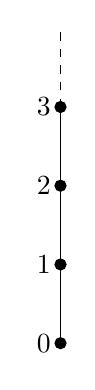
\begin{tikzpicture}
		\filldraw[black] (0,0) circle (2pt) node[anchor=east]{0};
		\filldraw[black] (0,1) circle (2pt) node[anchor=east]{1};
		\filldraw[black] (0,2) circle (2pt) node[anchor=east]{2};
		\filldraw[black] (0,3) circle (2pt) node[anchor=east]{3};
		\draw[black] (0,0)--(0,1);
		\draw[black] (0,1)--(0,2);
		\draw[black] (0,2)--(0,3);
		\draw[dashed,black] (0,3)--(0,4);
	\end{tikzpicture}
\captionof{figure}{Diagramma di Hasse dell'insieme totalmente ordinato $(\mathbb{N},\leq)$}
\end{center}

\begin{example}
	 Si consideri l'insieme $S=\{1,2,3\}$ con la relazione d'ordine usuale. Il diagramma \ref{fig:hasse2} non rappresenta un diagramma di Hasse in quanto $1 \cancel{\lessdot} 3$. Infatti: $] 1,3[ = \{2\} \neq \varnothing$.
	
	\begin{center}
		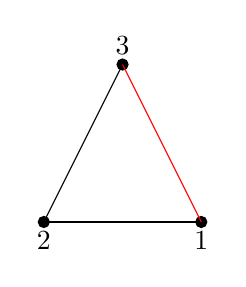
\begin{tikzpicture}
				\filldraw[black] (0,0) circle (2pt) node[anchor=south]{$3$};
				\filldraw[black] (-1,-2) circle (2pt) node[anchor=north]{$2$};
				\filldraw[black] (1,-2) circle (2pt) node[anchor=north]{$1$};
				
				\draw[black] (0,0)--(-1,-2);
				\draw[black] (-1,-2) -- (1,-2);
				\draw[red] (1,-2) -- (0,0);
		\end{tikzpicture}
			\captionof{figure}{}\label{fig:hasse2}
	\end{center}
\end{example}

\begin{example}
	Si consideri l'insieme $S=\{1,2,3\}$ ordinato mediante la relazione identica, o d'uguaglianza $id_{S}$. Chiaramente ogni elemento, essendo diverso da ogni altro elemento dell'insieme, sarà in relazione solo con se stesso. IL diagramma di Hasse che ne deriva prende il nome di \textbf{anticatena}:
	\medskip
	
	\begin{center}
		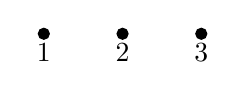
\begin{tikzpicture}
			\filldraw[black] (0,0) circle (2pt) node[anchor=north]{1};
			\filldraw[black] (1,0) circle (2pt) node[anchor=north]{2};
			\filldraw[black] (2,0) circle (2pt) node[anchor=north]{3};
		\end{tikzpicture}
	\end{center}
\end{example}

\begin{example}
	Le classi in \texttt{java.util} ordinate mediante la relazione gerarchica formano un insieme parzialmente ordinato in quanto non tutte le classi sono in relazione tra di loro (ad esempio \texttt{Vector} e \texttt{HashSet}). Si ottiene il seguente diagramma delle classi che non è altro che un diagramma di Hasse dell'insieme ordinato:
	\begin{center}
		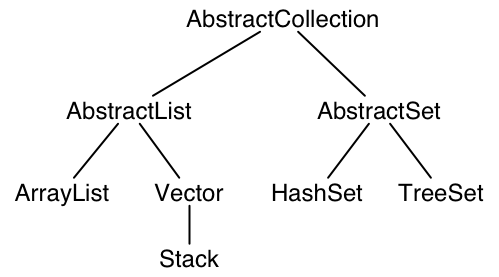
\includegraphics[scale=.35]{res/pojavautil.png}
	\end{center}
\end{example}
\begin{example}
\begin{enumerate}
		\item  Si consideri l'insieme ordinato $(\mathcal{P}(I_{n}), \subseteq)$ nel caso in cui $I_{n}$ sia l'insieme vuoto, $I_{n}$ abbia un solo elemento, due e tre elementi. Ricordiamo che $I_{n} = \{x \in \mathbb{N} \ | \ x \leq n\}$. Si ottengono quindi i diagrammi mostrati in Figura:
	
	\begin{center}
		\begin{minipage}{.1\textwidth}
			
\begin{tikzpicture}
				\filldraw[black] (5,0) circle (2pt) node[anchor=west]{$\varnothing$};
			\end{tikzpicture}
		\end{minipage}
		\begin{minipage}{.1\textwidth}
			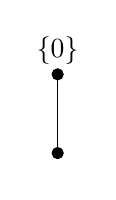
\begin{tikzpicture}
				\filldraw[black] (0,0) circle (2pt) node[anchor=south]{$\{0\}$};
				\filldraw[black] (0,-1) circle (2pt) node[anchor=north]{$\varnothing$};
				\draw[black] (0,0)--(0,-1);
			\end{tikzpicture}
		\end{minipage}
		\begin{minipage}{.25\textwidth}
			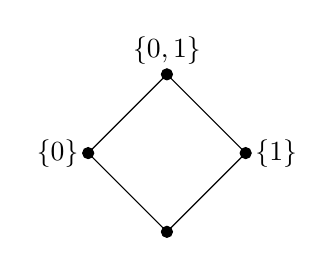
\begin{tikzpicture}
				\filldraw[black] (0,1) circle (2pt) node[anchor=south]{$\{0,1\}$};
				\filldraw[black] (-1,0) circle (2pt) node[anchor=east]{$\{0\}$};
				\filldraw[black] (1,0) circle (2pt) node[anchor=west]{$\{1\}$};
				\filldraw[black] (0,-1) circle (2pt) node[anchor=north]{$\varnothing$};
				
				\draw[black] (0,1)--(-1,0);
				\draw[black] (-1,0) -- (0,-1);
				\draw[black] (0,-1) -- (1,0);
				\draw[black] (1,0) -- (0,1);
			\end{tikzpicture}
		\end{minipage}
		\begin{minipage}{.45\textwidth}
			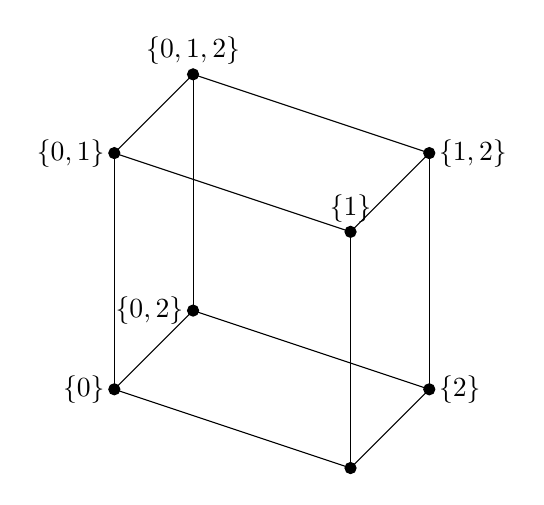
\begin{tikzpicture}
				\filldraw[black] (1,2) circle (2pt)node[anchor=south]{$\{0,1,2\}$};
				\filldraw[black] (0,1) circle (2pt)node[anchor=east]{$\{0,1\}$};
				\filldraw[black] (4,1) circle (2pt)node[anchor=west]{$\{1,2\}$};
				\filldraw[black] (3,0) circle (2pt)node[anchor=south]{$\{1\}$};
				\filldraw[black] (1,-1) circle (2pt)node[anchor=east]{$\{0,2\}$};
				\filldraw[black] (4,-2) circle (2pt)node[anchor=west]{$\{2\}$};
				\filldraw[black] (3,-3) circle (2pt)node[anchor=west]{$\varnothing$};
				\filldraw[black] (0,-2) circle (2pt)node[anchor=east]{$\{0\}$};
				\draw[black] (1,2)--(0,1);
				\draw[black] (0,1) -- (0,-2);
				\draw[black] (1,2) -- (4,1);
				\draw[black] (4,1) -- (4,-2);
				\draw[black] (3,0) -- (4,1);
				\draw[black] (0,1) -- (3,0);
				\draw[black] (0,-2) -- (3,-3);
				\draw[black] (3,-3) -- (4,-2);
				\draw[black] (1,2) -- (1,-1);
				\draw[black] (3,-3) -- (3,0);
				\draw[black] (1,-1) -- (4,-2);
				\draw[black] (0,-2) -- (1,-1);
			\end{tikzpicture}
		\end{minipage}
	\end{center}

\item 	Consideriamo l'insieme $Div(36)=\{1,2,3,4,6,9,12,18,36\}$ ordinato secondo la divisibilità. Il suo diagramma di Hasse è:
	\begin{center}
		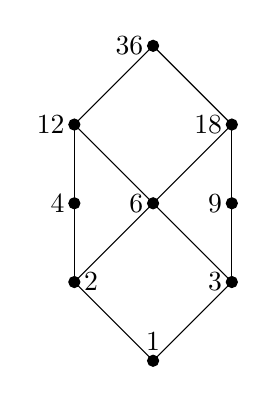
\begin{tikzpicture}
			\filldraw[black] (2,0) circle (2pt)node[anchor=south]{1};
			\filldraw[black] (1,1) circle (2pt)node[anchor=west]{2};
			\filldraw[black] (3,1) circle (2pt)node[anchor=east]{3};
			\filldraw[black] (1,2) circle (2pt)node[anchor=east]{4};
			\filldraw[black] (2,2) circle (2pt)node[anchor=east]{6};
			\filldraw[black] (3,2) circle (2pt)node[anchor=east]{9};
			\filldraw[black] (1,3) circle (2pt)node[anchor=east]{12};
			\filldraw[black] (3,3) circle (2pt)node[anchor=east]{18};
			\filldraw[black] (2,4) circle (2pt)node[anchor=east]{36};
			\draw[black] (2,0)--(1,1);
			\draw[black] (2,0)--(3,1);
			\draw[black] (1,1)--(1,2);
			\draw[black] (1,1)--(2,2);
			\draw[black] (3,1)--(2,2);
			\draw[black] (3,1)--(3,2);
			\draw[black] (2,2)--(1,3);
			\draw[black] (2,2)--(3,3);
			\draw[black] (1,2)--(1,3);
			\draw[black] (3,2)--(3,3);
			\draw[black] (1,3)--(2,4);
			\draw[black] (3,3)--(2,4);
		\end{tikzpicture}
	\end{center}
\end{enumerate}
\end{example}



\begin{osservation}
	Due insiemi si dicono \textbf{isomorfi} se hanno lo stesso diagramma di Hasse. Il duale di un diagramma di Hasse (ovvero il diagramma di Hasse della sua relazione opposta) si ottiene ruotando il grafico di 180°.
\end{osservation}

\begin{example}
	Consideriamo l'insieme ordinato $(\mathbb{N},\divides)$ e costruiamone il diagramma di Hasse (parziale):
	\begin{center}
		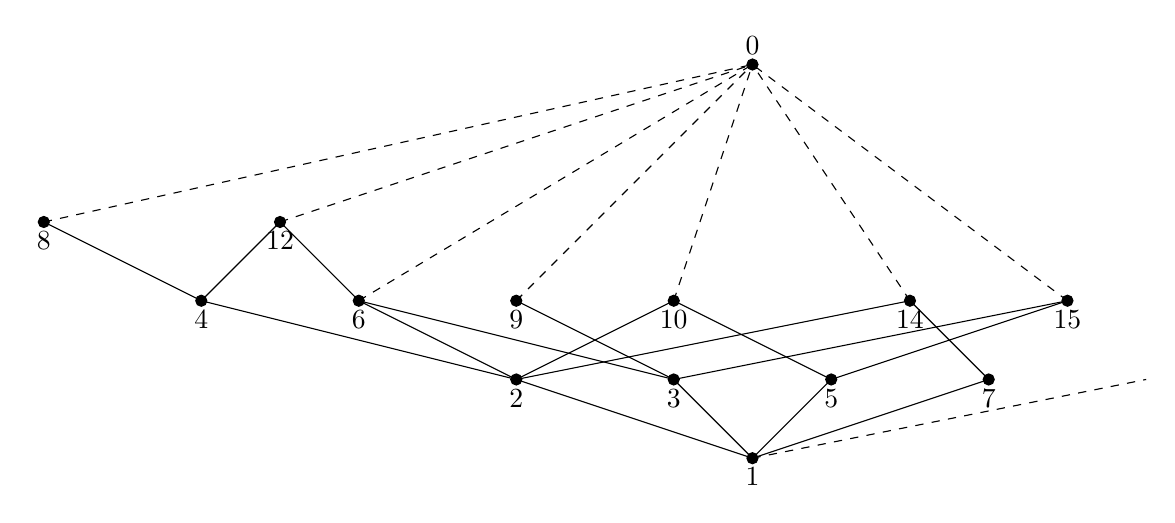
\begin{tikzpicture}
			\filldraw[black] (0,0) circle (2pt)node[anchor=north]{1};
			\filldraw[black] (-3,1) circle (2pt)node[anchor=north]{2};
			\filldraw[black] (-1,1) circle (2pt)node[anchor=north]{3};
			\filldraw[black] (1,1) circle (2pt)node[anchor=north]{5};
			\filldraw[black] (3,1) circle (2pt)node[anchor=north]{7};
			\draw[black] (0,0)--(-3,1);
			\draw[black] (0,0)--(-1,1);
			\draw[black] (0,0)--(1,1);
			\draw[black] (0,0)--(3,1);
			\draw[dashed] (0,0)--(5,1);
			\filldraw[black] (-7,2) circle (2pt)node[anchor=north]{4};
			\filldraw[black] (-5,2) circle (2pt)node[anchor=north]{6};
			\filldraw[black] (-3,2) circle (2pt)node[anchor=north]{9};
			\filldraw[black] (-1,2) circle (2pt)node[anchor=north]{10};
			\filldraw[black] (2,2) circle (2pt)node[anchor=north]{14};
			\filldraw[black] (4,2) circle (2pt)node[anchor=north]{15};
			\draw[black] (-3,1) --(-7,2);
			\draw[black] (-3,1) --(-5,2);
			\draw[black] (-3,1) --(-1,2);
			\draw[black] (-3,1) --(2,2);
			\draw[black] (-1,1)--(-5,2);
			\draw[black] (-1,1)--(-3,2);
			\draw[black] (-1,1)--(4,2);
			\draw[black] (1,1)--(-1,2);
			\draw[black] (1,1)--(4,2);
			\draw[black] (3,1)--(2,2);
			\filldraw[black] (-9,3) circle(2pt) node[anchor=north]{8};
			\filldraw[black] (-6,3) circle(2pt) node[anchor=north]{12};
			\draw[black] (-7,2)--(-9,3);
			\draw[black] (-7,2)--(-6,3);
			\draw[black] (-5,2)--(-6,3);
			\filldraw[black] (0,5) circle (2pt) node[anchor=south]{0};
			\draw[dashed](-9,3)--(0,5);
			\draw[dashed](-6,3)--(0,5);
			\draw[dashed](-5,2)--(0,5);
			\draw[dashed](-3,2)--(0,5);
			\draw[dashed](-1,2)--(0,5);
			\draw[dashed](2,2)--(0,5);
			\draw[dashed](4,2)--(0,5);
		\end{tikzpicture}
	\captionof{figure}{Diagramma di Hasse dell'insieme ordinato $(\mathbb{N},\divides)$.}\label{fig:hasse_n_divides}
	\end{center}
\end{example}

\subsection{Maggioranti, minoranti, estremo superiore ed inferiore}

\begin{defbox}{Maggioranti e minoranti}
	Sia $(S, \leq)$ un insieme ordinato, e sia $X$ una parte non vuota di $S$. Un elemento $a \in S$ si dice \textbf{minorante} di $X$ se risulta $a \leq x$ per ogni $x$ in $X$. Si dice invece che $a$ è un \textbf{maggiorante} di $X$ se $x \leq a$ per ogni $x \in X$.
\end{defbox}

\begin{defbox}{Insiemi inferiormente e superiormente limitati}
	Una parte $X\subseteq S$ si dice \textbf{inferiormente limitata} se è dotata di minoranti, mentre $X$ si dice \textbf{superiormente limitata} se è dotata di maggioranti.
\end{defbox} 

L'insieme dei minoranti di $X$ si denota col simbolo:
\begin{equation}
	X^{\downarrow}_{(S,\leq)}=\{a \in S \ | \ \forall x \in X (a \leq x)\}
\end{equation}
Mentre l'insieme dei maggioranti si denota col simbolo:
\begin{equation}
	X^{\uparrow}_{(S,\leq)}=\{a \in S \ | \ \forall x \in X (x \leq a)\}
\end{equation}


\begin{example}
	Si consideri il seguente diagramma di Hasse:
	\begin{center}
		\begin{tikzpicture}
			\filldraw[black] (1,1) circle (2pt) node[anchor=east]{c};
			\filldraw[black] (0,0) circle (2pt) node[anchor=east]{d};
			\filldraw[black] (2,0) circle (2pt) node[anchor=east]{e};
			\filldraw[black] (0,-2) circle (2pt) node[anchor=east]{a};
			\filldraw[black] (2,-2) circle (2pt)node[anchor=west]{b};
			\filldraw[black](1,-3) circle (2pt)node[anchor=north]{f};
			\filldraw[black](3,-1) circle (2pt)node[anchor=east]{g};
			\node[shape=ellipse,minimum height=1cm,draw=blue,fit={(0,-2)(2,-2)}]{};
			\draw[black] (1,1)--(0,0);
			\draw[black] (1,1)--(2,0);
			\draw[black] (2,0)--(0,-2);
			\draw[black] (0,0)--(0,-2);
			\draw[black] (0,-2)--(1,-3);
			\draw[black] (1,-3)--(3,-1);
			\draw[black] (2,-2)--(1,-3);
			\draw[black] (2,0)--(2,-2);
		\end{tikzpicture}
	\end{center}
	Si ha che l'insieme dei maggioranti di $\{a,b\}$ è dato da:
	\begin{displaymath}
		\{a,b\}^{\uparrow} =\{c,e\}
	\end{displaymath}
	mentre l'insieme dei minoranti di $\{a,b\}$ è:
	\begin{displaymath}
		\{a,b\}^{\downarrow} = \{f\}
	\end{displaymath}
\end{example}

\begin{example}
	Sia $(\mathcal{P}(S),\subseteq)$ allora, per un sottoinsieme $X \subseteq S$:
	\begin{eqnarray}
			X^{\uparrow} &= \{ Y \in \mathcal{P}(S) \; | \; \forall c \in \bigcup X (c \in Y) \} = \{Y \in \mathcal{P}(S) \; | \; \bigcup X \subseteq Y \}\\
			X^{\downarrow} &= \{Y \in \mathcal{P}(S) \; | \; \forall x \in X (Y \subseteq x )\} = \begin{cases}
				\{Y \in \mathcal{P}(S) \; | \; Y \subseteq \bigcap X\} & \text{se $X \neq \emptyset$}\\
				\{Y \; | \; Y \in \mathcal{P}(S) \} = \mathcal{P}(S) & \text{se $X= \emptyset$}
			\end{cases}
	\end{eqnarray}
Sia $S= \mathbb{N}$ e sia $X= \{\{1,2\},\{2,3\}\}$. Allora:
\begin{align*}
	X^{\uparrow} &=& \{Y \in \mathcal{P}(\mathbb{N}) \; | \; \bigcup X \subseteq Y \} = \{Y 	\in \mathcal{P}(\mathbb{N}) \; | \; \{1,2,3\} \subseteq Y \}\\
	X^{\downarrow} &=& \{Y \in \mathcal{P}(\mathbb{N})\; | \; Y \subseteq \bigcap X\} = \{Y \in \mathcal{P}(\mathbb{N}) \; | \; Y \subseteq \{2\} \} = \{\emptyset, \{2\}\}
\end{align*}
\end{example}

\begin{defbox}{Estremo inferiore e superiore}
	Sia $(S,\leq)$ un insieme ordinato, e sia $X$ una parte inferiormente limitata di $S$. Allora l'insieme dei minoranti di $X$ è una parte non vuota di $S$, il cui eventuale massimo di chiama \textbf{estremo inferiore} di $X$ e si denota col simbolo $inf_{(S,\leq)} X$. Se invece $X$ è una parte superiormente limitata di $S$, l'eventuale minimo dell'insieme dei maggioranti di $X$ si chiama \textbf{estremo superiore} di $X$ e si denota col simbolo $sup_{(S,\leq)} X$:
	\begin{eqnarray}
		inf_{(S,\leq)} X = max(X^{\downarrow}_{(S,\leq)})\\
		sup_{(S,\leq)} X = min(X^{\uparrow}_{(S,\leq)})
	\end{eqnarray}
\end{defbox}

\begin{example}
	Sia $X = \{C \in \mathcal{P}(\{1,2,3,4,5,6\}) \; | \; |C| \text{ è pari} \}$, ordinato mediante l'inclusione. Sia $A = \{\{1,2\},\{1,3\},\{2,5\}\} \subseteq X$. Allora abbiamo $A^{\downarrow} = \{\emptyset\}	$ e $A^{\uparrow}=\{\{1,2,3,5\},\{1,2,3,4,5,6\}\}
	$. Dunque:
\begin{align*}
	inf(A) &= max(A^{\downarrow}) = \emptyset\\
	sup(A) &= min(A^{\uparrow}) = \{1,2,3,5\}
\end{align*}
\end{example}

\begin{osservation}
	Se $S$ è un insieme ordinato non costituito da un solo elemento, nell'insieme ordinato $(\mathcal{P}(S)\setminus\{\varnothing\}, \subseteq)$ gli elementi minimali sono i sottoinsiemi del tipo $\{x\}$, con $x \in S$. Similmente, è chiaro che se l'insieme ordinato $S$ è dotato di massimo, questo è \textit{l'unico elemento massimale}. D'altra parte, qualunque sia l'insieme $S$ non costituito da un solo elemento, per ogni $x \in S$ il sottoinsieme $S \setminus \{x\}$ è un elemento massimale dell'insieme ordinato $(\mathcal{P}(S)\setminus \{S\}, \subseteq)$.
\end{osservation}

\begin{teorbox}
	Sono equivalenti le seguenti affermazioni:
	\begin{enumerate}
		\item $a \leq b$
		\item $a = min \{a,b\}$
		\item $a = inf\{a,b\}$
		\item $a \in \{a,b\}^{\downarrow}$
	\end{enumerate}
\end{teorbox}

\begin{osservation}
	Riprendiamo il Diagramma di Hasse dell'insieme ordinato $(\mathbb{N},\divides)$ (Figura \ref{fig:hasse_n_divides}). Per ogni coppia $(a,b)$ vale:
	\begin{eqnarray}
		inf(\{a,b\}) = MCD(a,b) \\
		sup(\{a,b\}) = mcm(a,b)
	\end{eqnarray}
Infatti, il massimo comun divisore di $a$ e $b$ è il più grande numero che divide $a$ e $b$, ovvero risulta essere il massimo dei minoranti secondo la relazione di divisibilità. Analogamente, il minimo comune multiplo risulta essere il minimo dell'insieme dei maggioranti (i multipli comuni di $a$ e $b$ per l'appunto).
\end{osservation}

\begin{example}
	Sia $(A,\leq)$ l'insieme ordinato definito dal diagramma di Hasse mostrato in Figura \ref{fig:example_inf_sup} e sia $B=\{c,d,e\}$:
	\begin{center}
		\begin{tikzpicture}
			\filldraw[black] (.5,2.5)circle (2pt) node[anchor=south]{a};
			\filldraw[black] (4,2.5) circle (2pt) node[anchor=south]{b};
			\filldraw[black] (2,1.5) circle (2pt) node[anchor=south]{c};
			\filldraw[black] (1,1) circle (2pt) node[anchor=south]{d};
			\filldraw[black] (3,1) circle (2pt) node[anchor=south]{e};
			\filldraw[black] (2,0) circle (2pt) node[anchor=south]{f};
			\filldraw[black] (4.5,.5) circle (2pt) node[anchor=south]{g};
			\node[shape=ellipse,draw=blue,fit={(2,1.5)(1,1)(3,1)}]{};
			\draw[black,thin] (2,0)--(1,1);
			\draw[black,thin] (2,0)--(3,1);
			\draw[black,thin] (4.5,.5)--(3,1);
			\draw[black,thin] (1,1)--(2,1.5);
			\draw[black,thin] (2,1.5)--(3,1);
			\draw[black,thin] (2,1.5)--(.5,2.5);
			\draw[black,thin] (2,1.5)--(4,2.5);
		\end{tikzpicture}
		\captionof{figure}{}\label{fig:example_inf_sup}
	\end{center}
	L'insieme dei maggioranti di $B$ è: $$B^{\uparrow} = \{a,b,c\}$$ e risulta $sup \ B = c$ poiché $c \in B$, $c$ è l'elemento massimo di $B$. L'insieme dei minoranti di $B$ è $ \{ f \} $ e quindi $inf \ B = f$ . Poiché $f \notin B$ allora non esiste il minimo di $B$. Osserviamo che $g$ non precede $d$ e quindi non è un minorante di $B$.
\end{example}

\begin{example}
	Sia $(A,\leq)$ l'insieme ordinato definito dal diagramma di Hasse in Figura \ref{fig:example_inf_sup2} e sia $B = \{d,e,f\}$. L'insieme dei maggioranti di $B$ è $$B^{\uparrow}=\{a,b,c\}$$ e risulta sup \ B = c. Poiché $c \notin B$ allora il massimo di $B$ non esiste. L'insieme dei minoranti di $B$ è $$B^{\downarrow} = \{f,h\} $$ e risulta $inf \ B = f$. Poiché $f \in B$, $f$ è l'elemento minimo di $B$ (osserviamo che $g$ non è un minorante di $B$.
	\begin{center}
		\begin{tikzpicture}
			\filldraw[black] (1,4)circle (2pt) node[anchor=south]{a};
			\filldraw[black] (3,4) circle (2pt) node[anchor=south]{b};
			\filldraw[black] (2,3) circle (2pt) node[anchor=south]{c};
			\filldraw[black] (1,2) circle (2pt) node[anchor=south]{d};
			\filldraw[black] (3,2) circle (2pt) node[anchor=south]{e};
			\filldraw[black] (2,1) circle (2pt) node[anchor=south]{f};
			\filldraw[black] (4,1) circle (2pt) node[anchor=south]{g};
			\filldraw[black](3,0) circle (2pt) node[anchor=south]{h};
			\node[shape=ellipse,draw=blue,fit={(3,2)(1,2)(2,1)}]{};
			\draw[black,thin](3,0)--(2,1);
			\draw[black,thin](3,0)--(4,1);
			\draw[black,thin](4,1)--(3,2);
			\draw[black,thin](3,2)--(2,3);
			\draw[black,thin](2,3)--(1,4);
			\draw[black,thin](3,0)--(2,1);
			\draw[black,thin](2,1)--(1,2);
			\draw[black,thin](1,2)--(2,3)--(3,4);
			\draw[black,thin](2,1)--(3,2);
		\end{tikzpicture}
		\captionof{figure}{}\label{fig:example_inf_sup2}
	\end{center}
\end{example}

\begin{example}
 Sia $(A,\leq)$ l'insieme ordinato definito dal diagramma di Hasse in Figura \ref{fig:example_inf_sup3} e sia $B=\{b,c,d\}$. L'insieme dei maggioranti di $B$ è $$B^{\uparrow}=\{a,b\}$$ e risulta $sup \ B = b$. Poiché $b \in B$, $b$ è il massimo di $B$. L'insieme dei minoranti di $B$ è $B^{\downarrow}=\{e,f\}$ Poiché gli elementi $e,f$ sono non confrontabili, $inf \ B$ non esiste.
	\begin{center}
		\begin{tikzpicture}
			\filldraw[black] (2.5,4)circle (2pt) node[anchor=south]{a};
			\filldraw[black] (2.5,3) circle (2pt) node[anchor=north]{b};
			\filldraw[black] (0,2) circle (2pt) node[anchor=south]{c};
			\filldraw[black] (5,2) circle (2pt) node[anchor=south]{d};
			\filldraw[black] (1,0) circle (2pt) node[anchor=north]{e};
			\filldraw[black] (4,0) circle (2pt) node[anchor=north]{f};
			\node[shape=ellipse,draw=blue,fit={(2.5,3)(0,2)(5,2)}]{};
			\draw[black](1,0)--(5,2)--(2.5,3)--(2.5,4);
			\draw[black](4,0)--(0,2)--(2.5,3);
			\draw[black]  (0,2)--(1,0);
			\draw[black]  (5,2)--(4,0);
		\end{tikzpicture}
		\captionof{figure}{}\label{fig:example_inf_sup3}
	\end{center}
\end{example}
\section{Reticoli}

\begin{defbox}{Reticolo}
	Sia $(S, \leq)$ un insieme parzialmente ordinato. $S$ si dice \textbf{reticolo} se e solo se:
	\begin{equation}
		\forall a,b \in S \bigl( \exists inf_{(S,\leq)}(\{a,b\}) \land \exists sup_{(S,\leq)}(\{a,b\})
	\end{equation}
\end{defbox}

\begin{example}
\begin{enumerate}
	\item Si consideri il seguente diagramma di Hasse:
	\begin{center}
		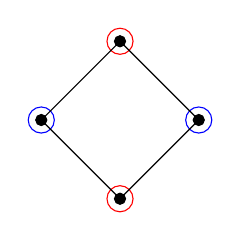
\begin{tikzpicture}
			\filldraw[black] (1,1) circle (2pt) node[shape = circle, minimum size=3pt, red, draw]{};
			\filldraw[black] (2,0) circle (2pt) node[shape = circle, blue, minimum size = 3pt, draw]{};
			\filldraw[black] (0,0) circle (2pt) node[shape = circle, blue, minimum size = 3pt, draw]{};
			\filldraw[black] (1,-1) circle (2pt) node[shape = circle, red, minimum size = 3pt, draw]{};
			\draw[black, thin] (1,1) -- (2,0)--(1,-1)--(0,0)--(1,1);
		\end{tikzpicture}
	\end{center}
	Per verificare che tale diagramma rappresenti un reticolo basterà osservare che le coppie non confrontabili (evidenziate in blu) abbiano sia un estremo superiore che un estremo inferiore (evidenziati in rosso).
	\item L'insieme dei numeri naturali, $\mathbb{N}$, ordinato mediante la divisibilità, è un reticolo.
	\item L'insieme $\{1,2,3,4,5,6,7,8,9\}$, ordinato mediante la divisibilità, non è un reticolo. Infatti, per esempio, $sup(\{6,9\})$ non esiste.
	\begin{center}
		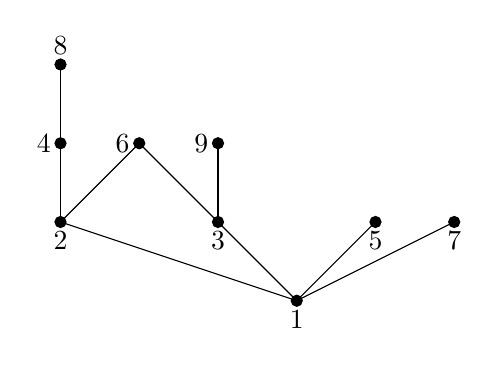
\begin{tikzpicture}
			\filldraw[black] (0,0) circle (2pt)node[anchor=north]{1};
			\filldraw[black] (-3,1) circle (2pt)node[anchor=north]{2};
			\filldraw[black] (-1,1) circle (2pt)node[anchor=north]{3};
			\filldraw[black] (-3,2) circle (2pt)node[anchor=east]{4};
			\filldraw[black] (1,1) circle (2pt)node[anchor=north]{5};
			\filldraw[black] (-2,2) circle (2pt)node[anchor=east]{6};
			\filldraw[black] (2,1) circle (2pt)node[anchor=north]{7};
			\filldraw[black] (-3,3) circle (2pt)node[anchor=south]{8};
			\filldraw[black] (-1,2) circle (2pt)node[anchor=east]{9};
			\draw[black] (0,0)--(-3,1);
			\draw[black] (0,0)--(-1,1);
			\draw[black] (0,0)--(1,1);
			\draw[black] (0,0)--(2,1);
			\draw[black] (-3,1)--(-2,2);
			\draw[black] (-3,1)--(-3,2);
			\draw[black] (-3,2)--(-3,3);
			\draw[black] (-1,1)--(-1,2);
			\draw[black] (-1,1)--(-2,2);
		\end{tikzpicture}
	\end{center}
	\item L'insieme $Div(36) = \{1,2,3,4,6,9,12,18,36\}$, ordinato mediante la divisibilità, è un reticolo. 
\end{enumerate}
\end{example}



\begin{propbox}
	Sia $(S,\leq)$ un reticolo e consideriamo $a \in S$. L'elemento $a$ è minimale in $S$ se e soltanto se $a = min(S,\leq)$. Dualmente per gli elementi massimali.
\end{propbox}

\begin{proof}
	\begin{itemize}
		\item[$\impliedby$] La condizione è chiaramente sufficiente. 
		\item[$\implies$] Sia $a$ un elemento minimale. Per ogni $b \in S$ poniamo $X = \{a,b\}$ e sia $c = inf (X) = max (X^{\downarrow})$, allora $c  \leq  a $ e $c \leq b$. Tuttavia, essendo $a$ minimale deve essere $c=a$ e quindi $a \leq b$ per ogni $b \in S$. Quindi, per definizione di minimo si ha l'asserto.
	\end{itemize}
\end{proof}

\begin{osservation}\label{oss:min_inf}
	Per ogni $a,b \in (S,\leq)\bigl( a \leq b \iff a = inf\{a,b\} \iff b= sup \{a,b\} \bigr)$. Inoltre, se $X \subseteq S$ ed esiste $x= inf(X)$ allora, essendo l'estremo inferiore il massimo dei minoranti, vale: $X^{\downarrow} = \{x\}^{\downarrow}$.
\end{osservation}

\begin{defbox}{Reticolo limitato e completo}
	Un reticolo si dice \textbf{limitato} se ammette minimo e massimo. Un reticolo si dice \textbf{completo} se ogni sua parte non vuota è dotata di estremo inferiore e superiore. Ogni reticolo completo è anche limitato.
\end{defbox}

\begin{osservation}
	Un reticolo finito non vuoto è sempre limitato. Il viceversa non vale: ci sono dei reticoli infiniti che sono limitati. Ad esempio se $A$ è un insieme infinito, $\mathcal{P}(A)$ è limitato, infatti si ha che il massimo di $\mathcal{P}(A)$ è $A$ stesso mentre il minimo è rappresentato dall'insieme vuoto. Il reticolo $(\mathbb{N},\leq)$ ha minimo, il numero naturale 0, ma non ha massimo. Quindi non è un reticolo limitato.
\end{osservation}


\begin{propbox}\label{prop_demorgan_minimali}
	Sia $(S,\rho)$ un insieme ordinato e siano $X,Y \subseteq S$ delle parti finite di $S$. Supponiamo che esistano $x= inf (X)$ e $y=inf(Y)$. Allora:
	\begin{align*}
		(X \cup Y )^{\downarrow} = X^{\downarrow} \cap Y^{\downarrow} = \{x\}^{\downarrow} \cap \{y\}^{\downarrow}
	\end{align*}
	Per dualità vale l'analogo per i maggioranti. Inoltre, se $(S,\rho)$ è un reticolo esiste $a=inf (\{x,y\}) = max(\{x,y\}^{\downarrow}) = max\bigl((X \cup Y)^{\downarrow}\bigr) = inf(X \cup Y)$.
\end{propbox}
\begin{proof}
	Sia $x \in (X \cup Y)^{\downarrow}$, valgono allora le seguenti equivalenze:
	\begin{align*}
		x \in (X \cup Y)^{\downarrow} &\iff \forall y \in X \cup Y (x\leq y) \\
		&\iff \forall y \bigl( (y \in X \lor y \in Y) \implies (x \leq y) \bigr) \\
		&\iff \forall y (y \in X \implies x \leq y) \land \forall y (y \in Y \implies x \leq y)\\
		&\iff x \in X^{\downarrow} \land x \in Y^{\downarrow}\\
		&\iff x \in X^{\downarrow} \cap Y^{\downarrow}
	\end{align*}
\end{proof}
\begin{corolbox}\label{corol:inf_sup}
	Sia $(S,\leq)$ un reticolo. Ogni sua parte finita è dotata di estremo inferiore e superiore.
\end{corolbox}
\begin{proof}
	Consideriamo una parte finita $T =\{a_{1},a_{2},\ldots,a_{n}\} \subset S$ e procediamo per induzione.
	\begin{itemize}
		\item Se $n=1$, cioè $T=\{a_{1}\}$, l'estremo inferiore di $T$ è semplicemente $a_{1}$ perché, per l'Osservazione \ref{oss:min_inf} si ha $T^{\downarrow}=\{a_{1}\}^{\downarrow}$, allora:
		\begin{align*}
			 inf(T)=max(T^{\downarrow}) = max(\{a_{1}\}^{\downarrow})=a_{1}
		\end{align*}
		\item Supponiamo che l'estremo inferiore esista per tutti i sottoinsiemi finiti di $S$ con $n$ elementi. Consideriamo un sottoinsieme con $n+1$ elementi, $T=\{a_{1},a_{2},\ldots,a_{n+1}\}$. Possiamo riscrivere $T$ come l'unione dell'insieme $T_{1}=\{a_{1},\ldots,a_{n}\}$ e $T_{2}=\{a_{1}\}$:
		\begin{align*}
			T = T_{1} \cup T_{2}
		\end{align*}
		Per ipotesi induttiva esiste l'estremo inferiore di $T_{1}$, sia esso $b = inf(\{a_{1},a_{2},\ldots,a_{n}\})$ ed, essendo $T_{2}$ un insieme di un solo elemento, risulta inoltre $inf(T_{2}) = a_{n+1}$. Per la Proposizione \ref{prop_demorgan_minimali} vale allora:
		\begin{align*}
			T^{\downarrow} &= (T_{1} \cup T_{2})^{\downarrow} \\
			&=T_{1}^{\downarrow} \cap T_{2}^{\downarrow} \\
			&= \{b\}^{\downarrow} \cap \{a_{n+1}\}^{\downarrow} \\
			&= \{b,a_{n+1}\}^{\downarrow}
		\end{align*}
	Dato che $S$ è un reticolo, l'insieme $\{b,a_{n+1}\}$ sicuramente ammette estremo inferiore, e vale quindi:
	\begin{displaymath}
		inf(\{b,a_{n+1}\}) = max(\{b,a_{n+1}\}^{\downarrow}) = max(T^{\downarrow}) = inf(T)
	\end{displaymath}
	\end{itemize}
\end{proof}

Se un insieme finito è un reticolo allora risulta essere un reticolo completo.

\subsection{Operazioni reticolari}
In questa sezione vedremo che i reticoli possono essere definiti, in modo equivalente, come insiemi muniti di due operazioni che soddisfano certe proprietà. L'idea è che $(a,b) \mapsto sup(\{a,b\})$ e $(a,b) \mapsto inf(\{a,b\})$ sono due operazioni che possiamo denotare rispettivamente $a \vee b$ e $a \wedge b$. Viceversa, la relazione d'ordine può essere ricavata da queste operazioni, nel modo seguente:
\begin{align*}
	\forall a,b \in S \bigl(	a \ \rho \ b \iff b = a \vee b 	\bigr)
\end{align*}
oppure:
\begin{align*}
	\forall a,b \in S \bigl(	a \ \rho \ b \iff a = a \wedge b 	\bigr)
\end{align*}

\begin{propbox}
	Sia $S$ un reticolo. Allora posto $a \vee b = sup(\{a,b\})$ e $a \wedge b = inf(\{a,b\})$, si ha che le operazioni su $S$:
	\begin{eqnarray}
		(a,b) \mapsto a \vee b \\
		(a,b) \mapsto a \wedge b	
	\end{eqnarray}
verificano le seguenti proprietà:
\begin{enumerate}
	\item \textit{Commutatività:} $a \vee b = b \vee a$ e $a \wedge b = b \wedge a$, per ogni $a,b \in S$;
	\item \textit{Associatività:} $a \vee (b \vee c) = (a \vee b) \vee c$ e $a \wedge (b \wedge c) = (a \wedge b) \wedge c$ per ogni $a,b,c \in S$
	\item \textit{Assorbimento:} $a \wedge ( a \vee b) = a$, $a \vee (a \wedge b) = a$, per ogni $a,b \in S$.
\end{enumerate}
\end{propbox}
\begin{proof}
	Evidente, la prova è lasciata al lettore come esercizio.
\end{proof}
\begin{osservation}
	Per ogni $a \in S$, $a$ è neutro rispetto a $\vee$ se e soltanto se, per ogni $b \in S$ si ha $b = a \vee b$. Cioè, se e soltanto se, $\forall b \in S (a \leq b)$ e cioè, $a = min(S,\leq)$. Dualmente, un elemento $a$ è neutro rispetto a $\vee$ se è il massimo di $(S,\leq)$. L'eventuale minimo di un reticolo si indica con il simbolo $0$ mentre l'eventuale massimo si indica con il simbolo 1.
\end{osservation}

Esaminiamo ora il viceversa della precedente Proposizione.
\begin{propbox}
	Sia $(S,\vee,\wedge)$ un insieme munito di due operazioni che verificano le proprietà:
	\begin{enumerate}
		\item \textit{Commutatività:} $a \vee b = b \vee a$ e $a \wedge b = b \wedge a$, per ogni $a,b \in S$;
		\item \textit{Associatività:} $a \vee (b \vee c) = (a \vee b) \vee c$ e $a \wedge (b \wedge c) = (a \wedge b) \wedge c$ per ogni $a,b,c \in S$
		\item \textit{Assorbimento:} $a \wedge ( a \vee b) = a$, $a \vee (a \wedge b) = a$, per ogni $a,b \in S$.
	\end{enumerate}
Allora la relazione $\rho$ su $S$ definita come:
\begin{equation}
	a \ \rho \ b \iff b = a \vee b
\end{equation}
è una relazione d'ordine su $S$. Si ha anche:
\begin{equation}\label{eq:wedge}
	a \ \rho \ b \iff a = a \wedge b
\end{equation}
Inoltre, $S$, munito di tale relazione d'ordine, è un reticolo, e, per ogni $a,b \in S$:
\begin{align*}
	\begin{cases*}
		sup(\{a,b\}) = a \vee b \\
		inf(\{a,b\}) = a \wedge b \\
	\end{cases*}
\end{align*}
\end{propbox}
\begin{proof}
	Iniziamo con il dimostrare la \ref{eq:wedge}. Infatti, se $a \ \rho \ b$, cioè se $b = a \vee b$, allora per l'assorbimento, $a \wedge b = a \wedge (a \vee b) = a$. Viceversa, se $a = a \wedge b$, ancora per l'assorbimento e per la commutatività, $a \vee b = (a \wedge b) \vee b = b \vee (a \wedge b) = b$.
	
	Dimostriamo ora che $\rho$ è una relazione d'ordine:
	\begin{enumerate}
		\item \textit{Riflessività:} $a \ \rho \ a$, cioè $a = a \vee a$. Infatti, usando le due proprietà di assorbimento, per ogni $a,b \in S$ si ha che $a = a \vee (a \wedge (a \vee b)) = a \vee a$;
		\item \textit{Antisimmetria:} Se $a \ \rho \ b$ e $b \ \rho \ a$, cioè se $b = a \vee b$ e $a = b \vee a $, allora, per la commutatività di $\vee$, deve essere $a=b$;
		\item \textit{Transitività:} se $a \ \rho \ b$ e $b \ \rho \ c$, cioè se $b= a \vee b$ e $c = b \vee c$ segue che $a \vee c = a \vee (b \vee c ) = (a \vee b) \vee c = a \vee c$.
	\end{enumerate}
	
	Rimane da dimostrare l'ultima asserzione. Dimostriamo che:
	\begin{align*}
		a \vee b = sup(\{a,b\})
	\end{align*}
Infatti, $a \ \rho \ (a \vee b)$, perché per la \ref{eq:wedge}, ciò è equivalente al fatto che $a \wedge ( a \vee b) = a$, cosa che è verificata per l'assorbimento. Allo stesso modo, si vede che $b \ \rho (a \vee b)$. Quindi $a \vee b$ è un maggiorante dell'insieme $\{a,b\}$ Rimane da dimostrare che è il minimo dell'insieme dei maggioranti. Supponiamo dunque che $a \ \rho \ c$ e $b \ \rho \ c$, cioè $c = a \vee c = b \vee c$. Allora $(a \vee b) \vee c = a \vee ( b \vee c) = a \vee c = c$, Dunque $(a \vee c) \ \rho \ c$ e l'asserzione è dimostrata. Il fatto che $ a \wedge b = inf(\{a,b\})$ si dimostra in modo analogo.
\end{proof}
\begin{defbox}{Reticolo come algebra}
Una struttura algebrica $(S,\wedge, \vee)$ a due operazioni interne si dice \textbf{reticolo} se le operazioni $\vee$ e $\wedge$ sono associative, commutative, e inoltre per ogni coppia $(a,b)$ di elementi di $S$ risulta:
\begin{eqnarray}\label{eq:assorbimento_meet_join}
	a \wedge(a \vee b) = a\\
	a \vee (a \wedge b)  = a
\end{eqnarray}
ovvero valgono le leggi di assorbimento. Se $(S,\wedge, \vee)$ è un reticolo, le operazioni $\wedge$ e $\vee$ sono spesso chiamate \textbf{intersezione} e \textbf{unione} in $S$ oppure \textbf{meet} e \textbf{join}.
\end{defbox}

\begin{example}
	Sia $X$ un qualunque insieme, e nell'insieme $\mathcal{P}(X)$ delle parti di $X$ si considerino le operazioni:
	\begin{align*}
		\cap: (A,B) \in \mathcal{P}(X)^{2} \mapsto A \cap B \in \mathcal{P}(X)
	\end{align*}
	e:
	\begin{align*}
		\cup: (A,B) \in \mathcal{P}(X)^{2} \mapsto A \cup B \in \mathcal{P}(X)
	\end{align*}
	Allora la terna $(\mathcal{P}(X),\cap,\cup)$ è un reticolo, chiamato \textbf{reticolo delle parti} di $X$.
\end{example}


\subsection{Sottoreticoli}
\begin{defbox}{Sottoreticolo}
	Sia $(S,\leq)$ un reticolo. Una parte $T \subseteq S$ si dice un \textbf{sottoreticolo} se esso è stabile rispetto a ciascuna delle operazioni reticolari $\wedge$ e $\vee$.
\end{defbox}

\begin{propbox}
	Gli intervalli chiusi di un reticolo sono sempre sottoreticoli.
\end{propbox}

\begin{proof}
	La dimostrazione è lasciata al lettore.
\end{proof}
È chiaro che un sottoreticolo è esso stesso un reticolo. Invece il viceversa non è necessariamente vero:  dato un reticolo $S$, esso può avere sottoinsiemi che sono reticoli rispetto alle operazioni di $S$ ma non sono sottoreticoli di $S$.
\begin{example}
	 Si consideri l'insieme $Div(12)=\{1,2,3,4,6,12\}$. Oltre ai \textbf{sottoreticoli banali} ($Div(12)$ stesso e i sottoinsiemi con un solo elemento) abbiamo i sottoreticoli $\{1,2,3,6\}$ e $\{2,4,6,12\}$. Sia $T=Div(12) \setminus \{2\} = \{1,3,4,6,12\} \subset Div(12)$.

	\begin{center}
		\begin{minipage}{.45\textwidth}
			\centering
			\begin{tikzpicture}
				\filldraw[black] (2,0) circle (2pt) node[anchor=north]{1};
				\filldraw[black] (0,1) circle (2pt) node[anchor=east]{3};
				\filldraw[black] (2,2) circle (2pt) node[anchor=south]{6};
				\filldraw[black] (4,1) circle (2pt) node[anchor=south]{2};
				\filldraw[black] (4,3) circle (2pt) node[anchor=south]{12};
				\filldraw[black] (6,2) circle (2pt) node[anchor=west]{4};
				\draw[black,thin] (2,0)--(0,1)--(2,2)--(4,1)--(6,2)--(4,3)--(2,2);
				\draw[black,thin] (2,0) --(4,1);
			\end{tikzpicture}
			\captionof{figure}{Il reticolo $(Div(12), \divides)$}
		\end{minipage}
		\hfil
		\begin{minipage}{.45\textwidth}
			\centering
			\begin{tikzpicture}
				\filldraw[black] (2,0) circle (2pt) node[anchor=north]{1};
				\filldraw[black] (0,1) circle (2pt) node[anchor=east]{3};
				\filldraw[black] (2,2) circle (2pt) node[anchor=south]{6};
				\filldraw[black] (4,3) circle (2pt) node[anchor=south]{12};
				\filldraw[black] (6,2) circle (2pt) node[anchor=west]{4};
				\draw[black,thin] (2,0)--(6,2)--(4,3)--(2,2)--(0,1)--(2,0);
			\end{tikzpicture}
			\captionof{figure}{Il reticolo $(Div(12) \setminus \{2\}, \divides)$}
		\end{minipage}
	\end{center}
 Chiaramente $T$ risulta essere un reticolo (perché per qualsiasi coppia di elementi esiste un estremo inferiore e superiore) ma non è un sottoreticolo di $(Div(12), \divides )$ in quanto non chiuso rispetto a $\wedge$, infatti:
 \begin{align*}
 	6 \wedge_{T} 4 = inf_{(T,\divides)}(\{6,4\}) =1 \neq 2 = inf_{(Div(12),\divides)}(\{6,4\}) = 6 \wedge_{Div(12)} 4
\end{align*}
\end{example}

\subsection{Omomorfismi tra reticoli}
Siano $(S_{1},\wedge,\vee)$ e $(S_{2},\wedge,\vee)$ reticoli. Seguendo la terminologia introdotta nella sezione \ref{sez:omomorfismi} un'applicazione $f: S_{1} \longrightarrow S_{2}$ si dice \textbf{omomorfismo}  se risulta, per ogni coppia $(a,b) \in S_{1}$:
\begin{displaymath}
	\begin{array}{lll}
		f(a \wedge b) = f(a) \wedge f(b), & & f(a \vee b) = f(a) \vee f(b)
	\end{array}
\end{displaymath}


\begin{teorbox}
	Siano $(S,\rho)$ e $(T, \sigma)$ due reticoli con operazioni reticolari $\wedge$, $\vee$ per $S$ e $\stackrel{\circ}{\wedge}$ e $\stackrel{\circ}{\vee}$ per $T$. Sia $f:S \rightarrow T$ una biezione. Allora $f$ è un isomorfismo tra i due insiemi ordinati se e soltanto se $f$ è un isomorfismo tra le strutture algebriche $(S,\wedge,\vee)$ e $(T,\stackrel{\circ}{\wedge} ,\stackrel{\circ}{\vee})$.
\end{teorbox}

\begin{proof}
	($\implies$) Per ogni $a,b \in S$ si ha $a \wedge b = inf_{(S,\rho)} (\{a,b\})$ e vale:
	\begin{displaymath}
		f(a \wedge b) = inf_{(T,\sigma)}\{f(a),f(b)\}=f(a) \stackrel{\circ}{\wedge} f(b)
	\end{displaymath}
	e dualmente $f(a \vee b) = f(a) \stackrel{\circ}{\vee} f(b)$. Quindi $f$ risulta essere un omomorfismo tra strutture algebriche e in particolare un isomorfismo.
	
	($\impliedby$) Per ipotesi, per ogni $a,b \in S$ si ha $f(a \wedge b) = f(a) \stackrel{\circ}{\wedge} f(b)$. Quindi:
	\begin{displaymath}
		a \leq b \iff a = a \wedge b \iff a = f(a \wedge b) = f(a) \stackrel{\circ}{\wedge} f(b) \iff f(a) \ \sigma \ f(b)
	\end{displaymath}
	ed $f$ risulta essere un isomorfismo tra i due insiemi ordinati.
\end{proof}

\subsection{Dualità reticolare}
\begin{defbox}{Relazione inversa}
	Siano $A,B$ due insiemi e sia $\sigma$ una corrispondenza tra $A$ e $B$. Definiamo la \textbf{relazione inversa} $\sigma^{-1}$ ponendo:
	\begin{displaymath}
		b \ \sigma^{-1} \ a \iff a \ \sigma \ b
	\end{displaymath}
\end{defbox}
\begin{propbox}{Principio di dualità}
	Se $\leq$ è una relazione d'ordine in $L$, allora $\leq^{-1}$ è ancora una relazione d'ordine. Inoltre, se $(L,\leq)$ è un reticolo, allora $(L,\leq^{-1})$ è ancora un reticolo.
\end{propbox}

\begin{defbox}{Reticolo duale}
	Sia $(L,\leq)$ un reticolo. Diciamo \textbf{reticolo duale} il reticolo $(L,\leq^{-1})$.
\end{defbox}

\subsection{Reticoli distributivi e complementati}

\begin{defbox}{Complemento}\label{def:complemento_reticolo}
	Sia $(S,\leq)$ un reticolo limitato. Un elemento $a \in S$ si dice un \textbf{complemento} di un elemento $b \in S$ se e solo se:
	\begin{displaymath}
		a \wedge b = min(S,\leq) = 0
	\end{displaymath}
	e
	\begin{displaymath}
		a \vee b = max(S,\leq) = 1
	\end{displaymath}
	Un reticolo si dice \textbf{complementato} se ogni elemento del reticolo ammette almeno un complemento.
\end{defbox}

\begin{example}
	Il reticolo delle parti di $S$ è un reticolo complementato infatti, presi $min \mathcal{P}(S) = \emptyset$ e $max \mathcal{P}(S)=S$, per ogni parte $X$ di $S$ si ha il complemento $S \setminus X$ e vale:
	\begin{displaymath}
		\begin{array}{l}
			X \wedge (S \setminus X)=inf \{X, S \setminus X\}= \emptyset \\
			X \vee (S \setminus X) = sup\{X, S \setminus X\} = S
		\end{array}
	\end{displaymath}
	Osserviamo inoltre che $\emptyset$ ed $S$ sono l'uno il complemento dell'altro ed è l'unico caso in cui due elementi $a,b$ sono sia complementari che confrontabili.
\end{example}

\begin{example}
	I reticoli:
	\begin{center}
		\begin{minipage}{.2\textwidth}
			\centering
			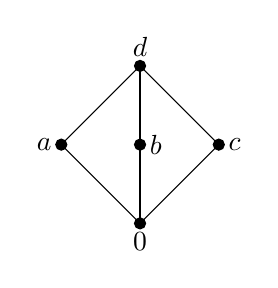
\begin{tikzpicture}
				\filldraw[black] (1,1) circle (2pt) node[above]{$d$};
				\filldraw[black] (0,0) circle (2pt) node[left]{$a$};
				\filldraw[black] (2,0) circle (2pt) node[right]{$c$};
				\filldraw[black] (1,0) circle (2pt) node[right]{$b$};
				\filldraw[black] (1,-1) circle (2pt) node[below]{$0$};
				\draw[-,thin] (1,1)--(0,0)--(1,-1)--(2,0)--(1,1);
				\draw[-,thin] (1,-1)--(1,0)--(1,1);
			\end{tikzpicture}
			\captionof{figure}{}\label{fig:reticolo1}
		\end{minipage}
		\hfil
		\begin{minipage}{.4\textwidth}
			\centering
			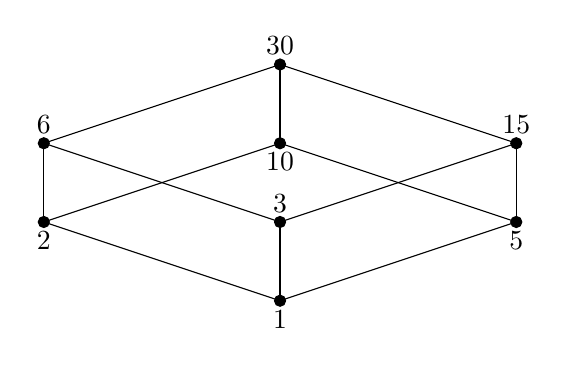
\begin{tikzpicture}
				\filldraw[black] (4,2) circle (2pt) node[below]{$10$};
				\filldraw[black] (4,3) circle (2pt) node[above]{$30$};
				\filldraw[black] (1,2) circle (2pt) node[above]{$6$};
				\filldraw[black] (4,1) circle (2pt) node[above]{$3$};
				\filldraw[black] (7,2) circle (2pt) node[above]{$15$};
				\filldraw[black] (1,1) circle (2pt) node[below]{$2$};
				\filldraw[black] (4,0) circle (2pt) node[below]{$1$};
				\filldraw[black] (7,1) circle (2pt) node[below]{$5$};
				\draw[-,thin] (4,2)--(7,1);
				\draw[-,thin] (7,2)--(7,1);
				\draw[-,thin] (7,1)--(4,0);
				\draw[-,thin] (1,1)--(1,2);
				\draw[-,thin] (1,2)--(4,3);
				\draw[-,thin] (1,2)--(4,1);
				\draw[-,thin] (4,1)--(7,2);
				\draw[-,thin] (4,2)--(1,1);
				\draw[-,thin] (4,2)--(4,3);
				\draw[-,thin] (4,3)--(7,2);
				\draw[-,thin] (1,1)--(4,0);
				\draw[-,thin] (4,1)--(4,0);
			\end{tikzpicture}
			\captionof{figure}{}\label{fig:reticolo2}
		\end{minipage}
		\hfil
		\begin{minipage}{.3\textwidth}
			\centering
			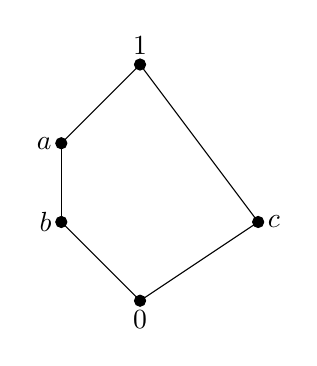
\begin{tikzpicture}
				\filldraw[black] (3,3) circle (2pt) node[above]{$1$};
				\filldraw[black] (2,2) circle (2pt) node[left]{$a$};
				\filldraw[black] (2,1) circle (2pt) node[left]{$b$};
				\filldraw[black] (3,0) circle (2pt) node[below]{$0$};
				\filldraw[black] (4.5,1) circle (2pt) node[right]{$c$};
				\draw[-,thin] (3,3)--(2,2);
				\draw[-,thin] (2,2)--(2,1);
				\draw[-,thin] (2,1)--(3,0);
				\draw[-,thin] (3,0)--(4.5,1);
				\draw[-,thin] (4.5,1)--(3,3);
			\end{tikzpicture}
			\captionof{figure}{}\label{fig:reticolo3}
		\end{minipage}
	\end{center}
	sono complementati. Nel caso del reticolo mostrato in Figura \ref{fig:reticolo1} l'elemento $a$ ha due complementi ($b$ e $c$) così come $b$ e $c$ hanno due complementi ciascuno. Analogamente, nel reticolo \ref{fig:reticolo3} l'elemento $c$ ha più di un complemento: $a$ e $b$ sono entrambi complementi di $c$ mentre $a$ e $b$ hanno entrambi un unico complemento ($c$). Nel caso del reticolo \ref{fig:reticolo2} ogni elemento ha un unico complemento. Notiamo inoltre che tale reticolo corrisponde all'insieme $Div(30)$ e che il complemento di ogni $k \in Div(30)$ corrisponde all'elemento $\frac{30}{k}$.
\end{example}

\begin{defbox}{Reticolo distributivo}
	Sia $(S,\wedge,\vee)$ un reticolo. Allora $(S,\leq)$ è \textbf{distributivo} se e soltanto se, per ogni $a,b,c \in S$:
	\begin{displaymath}
		\begin{array}{l}
			a \vee (b \wedge c) = (a \vee b) \wedge (a \vee c)\\
			a \wedge (b \vee c) = (a \wedge b) \vee (a \wedge c)
		\end{array}
	\end{displaymath}
	ossia $\wedge$ è distributiva rispetto a $\vee$ e viceversa.
\end{defbox}

\begin{example}
	Il reticolo delle parti di un insieme $S$ è distributivo in quanto $\cap$ e $\cup$ sono distributive l'una rispetto all'altra.
\end{example}


\begin{propbox}
	Se $(S,\leq)$ è un reticolo limitato distributivo, allora ogni $a \in S$ ammette unico complemento.
\end{propbox}


\begin{proof}
	Supponiamo per assurdo che $x$ e $y$ siano entrambi complementi di $a$ e sia $0= min S$ e $1= max S$. Allora:
	\begin{displaymath}
		\begin{array}{l}
			a \wedge x = 0 = a \wedge y \\
			a \vee x = 1 = a \vee y
		\end{array}
	\end{displaymath}
	Allora:
	\begin{displaymath}
		x = x \wedge 1 = x \wedge (a \vee y) = (x \wedge a) \vee (x \wedge y) = 0 \vee (x \wedge y) = x \wedge y
	\end{displaymath}
	Analogamente $y= y \wedge x$. Per la proprietà commutativa delle operazioni reticolari allora si ha $x=y$. 
\end{proof}

\begin{example}
	La distributività del reticolo è una condizione necessaria per l'unicità del complemento. Si consideri il seguente reticolo:
	\begin{center}
		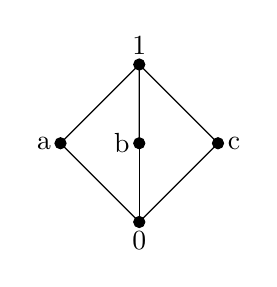
\begin{tikzpicture}
			\filldraw[black] (1,1) circle (2pt) node[anchor=south]{1};
			\filldraw[black] (0,0) circle (2pt) node[anchor=east]{a};
			\filldraw[black] (2,0) circle (2pt) node[anchor=west]{c};
			\filldraw[black] (1,-1) circle (2pt) node[anchor=north]{0};
			\filldraw[black] (1,0) circle (2pt) node[anchor=east]{b};
			\draw[-,thin] (1,0)--(1,1)--(0,0)--(1,-1)--(2,0)--(1,1);
			\draw[-,thin](1,0)--(1,-1);
		\end{tikzpicture}
	\end{center}
	Si ha chiaramente $\forall x(0 \leq x)$  e $\forall x (x \leq 1)$ ed inoltre i punti $a,b,c$ non sono confrontabili tra di loro. Allora chiaramente sia $b$ che $c$ sono dei complementi per $a$ ed infatti il reticolo non è distributivo:
	\begin{displaymath}
		a \vee (b \wedge c) = a \vee 0 = a
	\end{displaymath}
	mentre:
	\begin{displaymath}
		(a \vee b) \wedge (a \vee c) = 1 \wedge 1 = 1
	\end{displaymath}
	
	Inoltre, non è detto che se ogni elemento ha un unico complemento nel reticolo allora questo risulti distributivo. Non vale ovvero l'implicazione inversa.
	
\end{example}

\begin{defbox}{Reticolo pentagonale}
	Si consideri un insieme $X= \{x_{1},x_{2},x_{3},x_{4},x_{5}\}$ di ordine 5 e si introduca in $X$ una relazione d'ordine ponendo $\forall x \in X \bigl(x \leq x, \ x_{1} \leq x, \ x \leq x_{5} \bigr)$ e inoltre $x_{2} \leq x_{3}$. Allora $\{x_{2},x_{4}\}$ e $\{x_{3},x_{4}\}$ sono gli unici sottoinsiemi di ordine $2$ di $X$ costituiti da elementi non confrontabili, e si ha $x_{1}= inf\{x_{2},x_{4}\}=inf\{x_{3},x_{4}\}$ e $x_{5}=sup\{x_{3},x_{4}\}$ Il reticolo $(X,\wedge,\vee)$ associato all'insieme ordinato $(X,\leq)$ si chiama \textbf{reticolo pentagonale}.
\end{defbox}


\begin{defbox}{Reticolo trirettangolo}
	Sia $Y=\{y_{1},y_{2},y_{3},y_{4},y_{5}\}$ un altro insieme di ordine 5 e si introduca in $Y$ una relazione d'ordine $\leq$ ponendo $y \leq y$, $y_{1} \leq y$ e $y \leq y_{5}$ per ogni $y \in Y$. Allora $\{y_{2},y_{3}\}$, $\{y_{2},y_{4}\}$ e $\{y_{3},y_{4}\}$ sono i sottoinsiemi di ordine 2 di $Y$ costituiti da elementi non confrontabili, e si ha $y_{1}=inf\{y_{2},y_{3}\}=inf\{y_{2},y_{4}\}=inf\{y_{3},y_{4}\}$. Il reticolo $(Y,\wedge,\vee)$ associato all'insieme ordinato $(Y,\leq)$ si chiama \textbf{reticolo trirettangolo}.
\end{defbox}

	\begin{center}
\begin{minipage}{.45\textwidth}
	\centering
		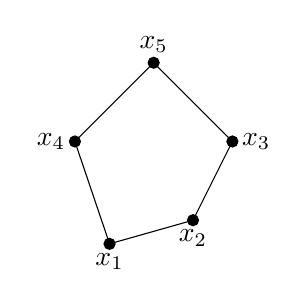
\begin{tikzpicture}
		\filldraw[black] (2,3) circle (2pt)node[anchor=south]{$x_{5}$};
		\filldraw[black] (3,2) circle (2pt)node[anchor=west]{$x_{3}$};
		\filldraw[black] (1,2) circle (2pt)node[anchor=east]{$x_{4}$};
		\filldraw[black] (1.44,0.7) circle (2pt) node[anchor=north]{$x_{1}$};
		\filldraw[black] (2.5,1) circle (2pt)node[anchor=north]{$x_{2}$};
		\draw[-,thin] (2,3)--(1,2)--(1.44,0.7)--(2.5,1)--(3,2)--(2,3);
	\end{tikzpicture}
\captionof{figure}{Reticolo pentagonale}
\end{minipage}
\hfil
\begin{minipage}{.45\textwidth}
	\centering
			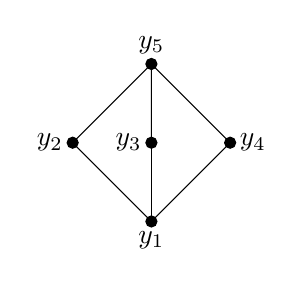
\begin{tikzpicture}
			\filldraw[black] (1,1) circle (2pt) node[anchor=south]{$y_{5}$};
			\filldraw[black] (0,0) circle (2pt) node[anchor=east]{$y_{2}$};
			\filldraw[black] (2,0) circle (2pt) node[anchor=west]{$y_{4}$};
			\filldraw[black] (1,-1) circle (2pt) node[anchor=north]{$y_{1}$};
			\filldraw[black] (1,0) circle (2pt) node[anchor=east]{$y_{3}$};
			\draw[-,thin] (1,0)--(1,1)--(0,0)--(1,-1)--(2,0)--(1,1);
			\draw[-,thin](1,0)--(1,-1);
		\end{tikzpicture}
	\captionof{figure}{Reticolo trirettangolo}
\end{minipage}
	\end{center}


Per capire se un reticolo è distributivo, ne costruisco il diagramma di Hasse e verifico se questo contiene un sottoreticolo pentagonale o trirettangolo. Se un reticolo li contiene, eredita a sua volta le proprietà dei sottoreticoli. Infatti, un reticolo isomorfo ad un altro reticolo ha le sue stesse proprietà. Vale quindi il seguente teorema.

\begin{teorbox}[Criterio di Birkhoff]\label{thm:birkhoff}
	Sia $(S,\leq)$ un reticolo, allora $(S,\leq)$ è distributivo se e soltanto se nessun sottoreticolo di $(S,\leq)$ è isomorfo ad un reticolo pentagonale o trirettangolo.
\end{teorbox}

\begin{corolbox}
	I reticoli pentagonali e trirettangolo sono i più piccoli tra i reticoli non distributivi. Ogni reticolo di ordine inferiore a 5 è distributivo.
\end{corolbox}

\pagebreak
\section{Strutture booleane}
\subsection{Anelli booleani}
\begin{defbox}{Anello booleano}
	Un anello $A$ si dice \textbf{booleano} se $A$ è unitario ed ogni elemento è idempotente, cioè coincide col proprio quadrato: $\forall a \in A \bigl(a = a \cdot a\bigr)$.
\end{defbox}

\begin{example}
	L'anello $(\mathcal{P}(S),\triangle,\cap)$ delle parti di un insieme è un anello booleano. Infatti è unitario e dal momento che l'operazione di moltiplicazione dell'anello $\mathcal{P}(S)$ è quella di intersezione, per ogni $X \in \mathcal{P}(S)$ si ha $X^{2}= X \cap X = X$.
\end{example}

\begin{defbox}{Caratteristica di un anello}
	Se $A$ è unitario e indichiamo l'unità di $A$ con $1_{A}$, se esiste qualche intero positivo $n \in \mathbb{Z^{+}}$ tale che:
	\begin{displaymath}
		n 1_{A} = 1_{A}+ 1_{A}+ \dots + 1_{A} = 0_{A}
	\end{displaymath}
	allora la \textbf{caratteristica} di $A$ è il minimo tale intero $n$.
\end{defbox}


\begin{osservation}
	Ovviamente $A$ ha caratteristica 1 se e soltanto se $1_{A}=0_{A}$ e quindi $A=\{0_{A}\}$. Altrettanto banale è il caso in cui la caratteristica di $A$ è due, per cui $1_{A} \neq 0_{A}$ e risulta $2 \cdot 1_{A}=0_{A}$. Notiamo che l'anello $(\mathcal{P}(S),\triangle, \cap)$ ha questa proprietà se $S \neq \emptyset$. Infatti in questo anello l'unità è $S$, lo zero è $\emptyset$, l'addizione è la differenza simmetrica e si ha $ 2 \cdot S = S \triangle S = \emptyset$. Quindi l'anello $\mathcal{P}(S)$ ha caratteristica 2.
\end{osservation}
Dimostriamo  ora che quanto appena visto per $(\mathcal{P}(S),\triangle, \cap)$ vale per tutti gli anelli booleani; verificando inoltre che questi anelli sono sempre commutativi.

\begin{propbox}
	Sia $A$ un anello booleano, allora $A$ è commutativo e, se $|A|>1$ allora $A$ ha caratteristica 2.
\end{propbox}

\begin{proof}
	Per ogni $a,b \in A$ vale: $a^{2}=a \cdot a = a$, $b^{2}= b \cdot b = b$. Quindi:
	\begin{align*}
		(a+b)^{2}&=(a+b)(a+b)\\
		&= a(a+b) + b(a+b)\\
		&= a^{2} + ab + ba + b^{2}\\
		&= a + ab + ba + b
	\end{align*}
	Essendo la caratteristica di $A$ pari a due, però, si ha che $(a+b)^{2}=(a+b)$ quindi:
	\begin{align*}
		a + ab + ba + b &= a+b \\
		&\implies ab+ba = 0_{A} \\
		&\implies ab = -ba
	\end{align*}
	Nel caso in cui sia $a=b$ si ottiene che, per ogni $a \in A$ vale $a^{2}=-a^{2}$ ovvero $a=-a$. Quindi $\forall a \in A$ si ha $2a = 0_{A}$. In particolare $2 \cdot 1_{A} = 0_{A}$, quindi o $1_{A}=0_{A}$ ed $A=\{0_{A}\}$ oppure $|A|>1$ e la caratteristica di $A$ è due. Infine, per ogni $a,b$, sfruttando $a=-a$ per l'elemento $ba$ si ha: $ba = -ba = ab$ ed $A$ risulta commutativo. 
\end{proof}

Enunciamo ma non dimostriamo il teorema di Stone, che è il risultato fondamentale nella teoria degli anelli booleani.

\begin{teorbox}[di Stone]
	Sia $A$ un anello booleano, allora:
	\begin{itemize}
		\item Esiste un insieme $S$ tale che $A$ sia isomorfo ad un sottoanello unitario di $(\mathcal{P}(S),\triangle,\cap)$;
		\item Se $A$ è finito esiste un insieme $S$ tale che $A$ sia isomorfo a $(\mathcal{P}(S),\triangle,\cap)$.
	\end{itemize}
\end{teorbox}

\begin{osservation}
	Tutti i sottoanelli unitari di $(\mathcal{P}(S),\triangle,\cap)$ sono booleani.
\end{osservation}


\begin{corolbox}
	Sia $R$ un anello booleano finito. Allora:
	\begin{enumerate}
		\item Esiste $n\in \mathbb{N}$ tale che $|R|=2^{n}$;
		\item Se $A$ è un anello booleano e $|A| = |R|$ allora $A \simeq R$.
	\end{enumerate}
\end{corolbox}

\begin{proof}
	Per il teorema di Stone, esiste un insieme $S$, ovviamente finito, tale che $R$ sia isomorfo a $(\mathcal{P}(S),\triangle,\cap)$. Posto $n=|S|$, allora $|R| = |\mathcal{P}(S)| = 2^{n}$, il che giustifica la (1). Se poi $A$ è un anello booleano, anch'esso di cardinalità $2^{n}$, ancora per il teorema di Stone abbiamo $A \simeq (\mathcal{P}(T),\triangle,\cap)$ per un opportuno insieme $T$. Ma allora $|\mathcal{P}(T)| = |A|$, quindi $|\mathcal{P}(T)|=2^{n}$ e deduciamo così $|T|=n$. Dunque $|T|=|S|$ e quindi $A \simeq R$.
\end{proof}

\subsection{Reticoli booleani}
Ricordiamo che un reticolo è un insieme ordinato non vuoto $(L,\leq)$ tale che, per ogni $a,b \in L$ esistano l'estremo inferiore $inf_{(L,\leq)}\{a,b\}$ e l'estremo superiore $sup_{(L,\leq)}\{a,b\}$ di $\{a,b\}$ in $(L,\leq)$. Ricordiamo anche che si può, in modo equivalente, riguardare i reticoli anche come strutture algebriche.

\begin{defbox}{Reticolo booleano}
	Un reticolo si dice \textbf{booleano} se e solo se è distributivo e complementato.
\end{defbox}

Come abbiamo appena visto, un reticolo può essere visto anche come una struttura algebrica $(L,\wedge,\vee)$. Affinché $L$ sia un reticolo booleano devono valere:
\begin{itemize}
	\item le proprietà commutative per $\wedge$ e $\vee$;
	\item le proprietà associative per $\wedge$ e $\vee$;
	\item le leggi di assorbimento;
	\item le proprietà distributive;
	\item l'esistenza degli elementi neutri di $\wedge$ e $\vee$ (ovvero devono esistere $min$ e $max$ del reticolo);
	\item ogni elemento deve avere un complemento. Esiste quindi l'applicazione\footnote{Che risulta ben posta in quanto il reticolo è distributivo e ogni elemento ammette un unico complemento.}: $': a \in L \mapsto a' \in L$.
\end{itemize}
Gli insiemi totalmente ordinati con massimo due elementi sono reticoli booleani.
\subsection{Algebre di Boole}
\begin{defbox}{Algebra di Boole}
	Si definisce \textbf{algebra di Boole} una struttura algebrica $(L,\vee,\wedge,0,1,')$ tale che:
	\begin{enumerate}
		\item $(L,\vee,0)$ e $(L,\wedge,1)$ sono monoidi commutativi;
		\item valgono le leggi di assorbimento: $\forall a,b \in L \bigl(a \vee(a \wedge b)=a=a\wedge(a \vee b)\bigr)$;
		\item vale la distributività di $\wedge$ rispetto a $\vee$ e viceversa;
		\item per ogni $a \in L$ esiste il complementare $a'$ per il quale $a \wedge a' = 0$ e $a \vee a'=1$.
	\end{enumerate}
	
\end{defbox}

\begin{osservation}
	Ogni reticolo booleano è un'algebra di Boole e viceversa. Infatti, la (1) e la (2) esprimono il fatto che $(L,\wedge,\vee)$ è un reticolo limitato, con minimo $0$ e massimo $1$ mentre la $(3)$ dice che questo reticolo è distributivo e la $(4)$ garantisce che ogni elemento $a$ di $L$ ha un complemento $a'$. Possiamo dunque dire che la nozione di algebra di Boole è la versione ``puramente algebrica'' della nozione di reticolo booleano.
\end{osservation}

\begin{defbox}{Sottoalgebra di Boole}
	Sia $(L,\vee,\wedge,0,1,')$ un'algebra di Boole. Un sottoinsieme $C \subset L$ è detto \textbf{sottoalgebra di Boole} se, per ogni $x,y \in C$:
	\begin{enumerate}
		\item $x \vee y \in C$ e $x \wedge y \in C$
		\item $0 \in C$ e $1 \in C$
		\item $x' \in C$
	\end{enumerate}
\end{defbox}

La nozione di sottoalgebra di Boole differisce da quella di sottoreticolo. Infatti, un sottoreticolo $K$ di un reticolo booleano $L$ deve essere chiuso rispetto alle due operazioni reticolari (quindi deve verificare la prima delle tre condizioni appena elencate), ma non contiene necessariamente il massimo o il minimo del reticolo né, tanto meno, i complementi dei suoi elementi.


\begin{example}
	\begin{enumerate}
		\item Sia $S \neq \emptyset$ un insieme. Consideriamo il reticolo booleano $(\mathcal{P}(S),\subseteq)$. Questo si struttura come algebra di Boole nella forma $(\mathcal{P}(S), \cup, \cap, \emptyset, S, \mathcal{C}_{X})$ dove $\mathcal{C}_{X}$ è l'applicazione ``complemento'' che manda ogni $X \in \mathcal{P}(S)$ in $S \setminus X$.
	
		\item Sia $\mathbb{B}=\{0,1\}$ dotato delle operazioni binarie $\wedge$ e $\vee$ e dell'operazione unaria $'$ dove:
		\begin{enumerate}
			\item $\vee$ (OR) è definita da $0\vee0 = 0$, $0 \vee 1=1 \vee 0 = 1 \vee 1 = 1$ ;
			\item $\wedge$ (AND) è definita da $0 \wedge 0 = 0 \wedge 1 = 1 \wedge 0 = $ e $1 \wedge 1 = 1$;
			\item $0'=1$ e $1'=0$.
		\end{enumerate}
		Si ha che $(\mathbb{B},\vee,\wedge,0,1,')$ è un'algebra di Boole.
	\end{enumerate}
\end{example}

Il prossimo enunciato elenca alcune identità che valgono nelle algebre di Boole. La terza si esprime dicendo che l’operazione di complemento è \textbf{involutoria}, cioè coincide con l’applicazione inversa di sé stessa (e, in particolare, è biettiva); le ultime due sono le note come leggi di De Morgan per algebre di Boole.

\begin{propbox}	
	Sia $(L,\vee,\wedge,0,1,')$ un'algebra di Boole. Allora $\forall a,b \in L$ valgono:
	\begin{enumerate}
		\item $1 \vee a = 1$ e $0 \wedge a = 0 $
		\item $1'=0 $ e $0' = 1$
		\item $(a')'=a $
		\item $(a \vee b)' = a' \wedge b' $
		\item $(a \wedge b)' = a' \vee b'$
	\end{enumerate}
\end{propbox}

\begin{proof}	
	La (1) e la (2) sono immediate in quanto $L$ è un reticolo.
	
	Per dimostrare la validità della (3) basta osservare che $a'$ è un complemento di $a$ e $a$ è un complemento di $a'$, anche $(a')'$ è un complemento di $a'$; quindi per l'unicità dei complementi nei reticoli booleani si ha $a=(a')'$.
	
	Per la $(4)$ basta mostrare che $(a' \wedge b')$ è un complemento di $a \vee b$, ovvero che:
	\begin{displaymath}
		(a \vee b) \vee (a' \wedge b') = 1
	\end{displaymath}
	e:
	\begin{displaymath}
		(a \vee b) \wedge (a' \wedge b') = 0
	\end{displaymath}
	Usando la distributività e la (1) si ottiene:
	\begin{align*}
		(a \vee b) \vee (a' \wedge b') &= (a \vee b \vee a') \wedge (a \vee b \vee b') \\
		&= (1 \vee b) \wedge (a \vee 1) \\
		&= 1 \wedge 1 = 1
	\end{align*}
	e
	\begin{align*}
		(a \vee b) \wedge (a' \wedge b') &= (a \wedge a' \wedge b') \vee (b \wedge a' \wedge b') = (0 \wedge b') \vee (0 \wedge a') \\
		&= 0 \vee 0 = 0
	\end{align*}
	La numero $(5)$ si dimostra in maniera duale.
\end{proof}

\subsection{Anelli booleani e algebre di Boole}

Si rimanda \href{https://www.dma.unina.it/cutolo/didattica/note/strutturebooleane.pdf}{qui} alle note del docente. Argomento cardine di questa sezione è la sostanziale \textit{equivalenza tra concetto di algebra di Boole, reticolo booleano e anello booleano} in quanto esiste una corrispondenza biunivoca fra le tre strutture, nel senso che si può costruire una struttura di reticolo booleano su ogni anello booleano e, viceversa, una struttura di anello booleano su ogni reticolo booleano, in modo che queste due
costruzioni siano l’una inversa dell’altra. Grazie al Teorema di Stone, infatti, ogni anello booleano finito è isomorfo a $(\mathcal{P}(S), \triangle, \cap)$ per un opportuno insieme $S$ (per gli anelli infiniti il teorema è un po' più debole: ogni anello booleano è isomorfo ad un sottoanello unitario di $(\mathcal{P}(S), \triangle, \cap)$, per un opportuno insieme $S$). Analoghi enunciati valgono per i reticoli booleani e per le algebre di Boole. 

In primo luogo, partendo da un anello booleano $(R,+,\cdot)$ vogliamo definire una struttura di reticolo booleano su $R$. L'esempio dell'anello delle parti di un insieme può suggerirci in che modo procedere. Fissato un insieme $S$, infatti, $(\mathcal{P}(S), \triangle, \cap)$ è un anello booleano ma $\mathcal{P}(S)$ è anche un reticolo booleano, con operazioni reticolari $\cup$ e $\cap$. La seconda operazione reticolare è proprio l'operazione di moltiplicazione nell'anello. Anche la prima operazione reticolare si può esprimere in termini delle operazioni dell'anello: per ogni $A,B \in \mathcal{P}(S)$ abbiamo infatti che:
\begin{displaymath}
	A \cup B = (A \triangle B) \cup (A \cap B) = (A \triangle B) \triangle (A \cap B)
\end{displaymath}
Inoltre, il minimo ed il massimo del reticolo sono $\emptyset$ e $S$, cioè lo zero e l'unità dell'anello, e ciascun $A \in \mathcal{P}(S)$ ha come complemento, nel reticolo $(\mathcal{P}(S),\subseteq)$ l'insieme $S \setminus A = S \triangle A = 1_{\mathcal{P}(S)} \triangle A$.

Passando ora ad un arbitrario anello booleano $(R,+,\cdot,0_{R},1_{R})$ dove $0_{R}$ e $1_{R}$ sono lo zero e l'unità dell'anello, l'esempio di $\mathcal{P}(S)$ suggerisce di definire in $R$ l'operazione binaria $\vee$ ponendo, per ogni $a,b \in R$:
\begin{equation}
	a \vee b \coloneqq a+b+ab
\end{equation}
e l'applicazione $':a \in R \mapsto 1_{R}+a \in R$ da utilizzare come operazione unaria di complemento.


\begin{propbox}
	Con le notazioni appena fissate, $(R,\vee, \cdot, 0_{R},1_{R},')$ è un'algebra di Boole.
\end{propbox}

\begin{proof}
	Dobbiamo verificare che $(R, \vee, 0_{R})$ e $(R, \cdot, 1_{R})$ siano monoidi commutativi, che valgano per $\vee$ e $\cdot$ le leggi di assorbimento e le proprietà distributive ed infine che l’applicazione $'$ verifichi la condizione richiesta dalla definizione di complemento.
	
	Che $\vee$ sia commutativa è evidente, ed è anche chiaro che $a \vee 0_{R} = a + 0_{R}+ a0_{R}$ per ogni $a \in R$, quindi $0_{R}$ è neutro rispetto a $\vee$. Proviamo l'associatività di $\vee$: per ogni $a,b,c \in R$ si ha:
	\begin{align*}
		(a \vee b) \vee c &= (a+b+ab) \vee c \\
		&= (a+b+ab) + c + (a+b+ab)c \\
		&= a+b+ab+c+ac+bc+abc
	\end{align*}
	Si ha inoltre:
	\begin{align*}
		a \vee (b \vee c) &= (b \vee c) \vee a \\
		&= b+c+a+bc+ba+ca+bca
	\end{align*}
	dunque $(a \vee b) \vee c = a \vee (b \vee c)$. È così provato che $\vee$ è associativa. $(R,\vee,0_{R})$ è un monoide commutativo. Che lo sia anche $(R,\cdot,1_{R})$ è già noto in partenza, dal momento che $R$ è un anello booleano.
	
	Verifichiamo le leggi di assorbimento. Per ogni $a,b \in R \bigl(a \vee (ab) = a +ab+a(ab) \bigr)$. Dal momento che $R$ è booleano, $a(ab) = a^{2}b = ab$ e $ab+ab=0_{R}$, quindi $a \vee  (ab) = a+ab+ab = a$. Inoltre $a(a \vee b) = a(a+b+ab) = a^{2}+ab+a^{2}b = a+ab+ab=a$. Le leggi di assorbimento sono così provate. A questo punto possiamo concludere che $(R,\vee,\cdot)$ è un reticolo limitato.
	
	Verifichiamo ora che $\cdot$ è distributiva rispetto a $\vee$. Per ogni $a,b,c \in R$ si ha $a(b \vee c) = a(b+c+bc)=ab+ac+abc$ e $(ab) \vee (ac) = ab+ac+(ab)(ac) = ab+ac+abc$. Dunque $a(b \vee c) = (ab) \vee (ac)$. Pertanto, utilizzando anche la proprietà commutativa, possiamo concludere che $\cdot$ è distributiva rispetto a $\vee$.
	
	Resta infine da dimostrare che, per ogni $a \in R$, l'immagine di $a$ mediante l'applicazione $'$, vale a dire $a' \coloneqq 1_{R}+a$, verifica le condizioni $a \vee (1_{R}+a)= 1_{R}$ e $aa' = 0_{R}$. Questo è molto facile: per ogni $a \in R$ si ha $aa'=a(1_{R}+a) = a+a = 0_{R}$ e $a \vee a' = a+a'+aa' = a+(1_{R}+a)+0_{R}=1_{R}$, come richiesto. Con questo la dimostrazione è completa. 
\end{proof}

Descriviamo ora la costruzione inversa: quella di un anello booleano a partire da un’algebra di Boole. Anche in questo caso ci facciamo guidare dall'esempio dell'algebra $(\mathcal{P}(S), \cup, \cap, \emptyset, S, \mathcal{C}_{X})$ delle parti di un insieme $S$. Delle due operazioni binarie dell'anello booleano $(\mathcal{P}(S),\triangle,\cap)$, quella di moltiplicazione, $\cap$, è già tra le operazioni dell'algebra di Boole. Per esprimere l'altra, la differenza simmetrica, utilizzando le operazioni dell'algebra di Boole ci è utile osservare che se $A$ e $B$ sono parti di $S$, allora $A \setminus B = A \cap (S \setminus B) = A \cap \mathcal{C}_{X}(B)$. Dunque $A \triangle B$ può essere scritta come:
\begin{displaymath}
	\begin{cases}
		(A \setminus B) \cup (B \setminus A)  = (A \cap \mathcal{C}_{X}(B)) \cup (B \cap \mathcal{C}_{X}(A)) \\
		(A \cup B ) \setminus (A \cap B) = (A \cup B) \cap (\mathcal{C}_{X}(A \cap B))
	\end{cases}
\end{displaymath}

Questo esempio mostra due modi possibili per definire, in un'arbitraria algebra di Boole, un'operazione binaria di addizione $+$ analoga alla differenza simmetrica in $\mathcal{P}(S)$.


\begin{lemmabox}
	Sia $(L,\vee,\wedge,0,1,')$ un'algebra di Boole. Allora, per ogni $a,b \in L$:
	\begin{displaymath}
		(a \wedge b') \vee (a' \wedge b) = (a \vee b) \wedge (a \wedge b) '
	\end{displaymath}
	
\end{lemmabox}
\begin{proof}
	Usando la proprietà distributiva di $\vee$ rispetto a $\wedge$ abbiamo:
	\begin{align*}
		(a \wedge b') \vee (a' \wedge b) &= (a \vee a') \wedge (a \vee b) \wedge (b' \vee a') \wedge (b' \vee b) \\
		&= 1 \wedge (a \vee b) \wedge (b' \vee a') \wedge 1 \\
		&= (a \vee b) \wedge (a' \vee b') \\
		&= (a \vee b) \wedge (a \wedge b)'
	\end{align*}
	avendo utilizzato, per ultimo passaggio, una delle leggi di De Morgan.
\end{proof}


\begin{teorbox}[di Stone per le algebre di Boole]
	Ogni reticolo booleano finito è isomorfo al reticolo finito delle parti. Ogni algebra di Boole è isomorfa ad un'algebra di Boole delle parti finite.
\end{teorbox}

Questo vuol dire, ad esempio, che se sappiamo descrivere il reticolo delle parti degli insiemi finiti, conosciamo, a meno di isomorfismi, tutti i reticoli booleani finiti. Una conseguenza del teorema di Stone è che gli anelli booleani finiti (ma lo stesso vale per i reticoli booleani finiti o per le algebre di Boole finite) hanno per cardinalità una potenza di 2, e che due anelli booleani finiti con lo stesso numero di elementi sono necessariamente isomorfi.

Sia allora $X \subseteq S$. Prendiamo la funzione caratteristica: \begin{displaymath}
\mbox{\Large$\chi$}_{X,S}: x \in S \mapsto \begin{cases*}
		0 & \text{ se} x \notin X \\
		1 & \text{ se} x \in X
	\end{cases*} \in \{0,1\}
\end{displaymath}
e alteriamone il codominio:
\begin{displaymath}
	\mbox{\Large$\chi$}_{X,S}: x \in S \mapsto \begin{cases*}
		\overline{0} & \text{ se} x \notin X \\
		\overline{1} & \text{ se} x \in X
	\end{cases*}
\in \mathbb{Z}_{2}
\end{displaymath}
Dimostriamo che $X \in \mathcal{P}(S) \mapsto \mbox{\Large$\chi$}_{X,S} \in Map(S,\mathbb{Z}_{2})$ è biettiva. Sia $S=\{1,2,3,\ldots,n\}$ con $n \in \mathbb{N}^{*}$. Allora $Map(S,\mathbb{Z}_{2})$ è l'insieme delle $n$-ple di elementi di $\mathbb{Z}_{2}$. Come già osservato, possiamo scrivere ogni funzione da $S$ in $\mathbb{Z}_{2}$ come una stringa $(s_{1}s_{2}\ldots s_{n})$. Chiamiamo $\mathbb{Z}_{2}^{n}$ l'insieme di tali stringhe, gli elementi di $\mathcal{P}(S)$ corrispondono quindi a tali stringhe.

Sia allora $R^{n} = R \times \cdots \times R$ il prodotto cartesiamo di $n$ copie di un anello $R$, ovvero l'insieme di $n$-ple di elementi di $R$. Se prendiamo due elementi e ne facciamo somma e prodotto, otteniamo:
\begin{align*}
	a+b = (a_{1}+b_{1}, a_{2}+b_{2}, \ldots, a_{n}+b_{n})\\
	a \cdot b = (a_{1}\cdot b_{1}, a_{2}\cdot b_{2}, \ldots, a_{n}\cdot b_{n})
\end{align*}
E possiamo considerare la struttura $(R^{n},+,\cdot)$ che risulta essere un anello. Se $R$ è booleano, anche $R^{n}$ è booleano. Allora anche $\mathbb{Z}_{2}^{n}$, per le stesse osservazioni, sarà un anello booleano rispetto alle operazioni di somma e prodotto.

\begin{example}
	Sia $S=\{1,2,3,4,5,6,7,8\}$ e consideriamo le stringhe $a=(10010011)$ e $b=(01101101)$, facendo somma e prodotto, otteniamo:
	\begin{align*}
		a+b = 1111 1110 = a \xor b\\
		a \cdot b = 0000 0001 = a \wedge b
	\end{align*}
dove $\xor$ e $\wedge$ sono i classici operatori logici bit a bit. Sappiamo inoltre che l'applicazione $X \in \mathcal{P}(S) \mapsto \mbox{\Large$\chi$}_{X,S} \in \mathbb{Z}_{2}^{8}$ è biettiva. Quindi prese le parti $A=\{1,4,7,8\}$ e $B=\{2,3,5,6,8\}$, codificate dalle stringhe $a=(10010011)$ e $b=(01101101)$, abbiamo:
\begin{align*}
	a+b =(11111110) = \{1,2,3,4,5,6,7\} = A \triangle B\\
	a \cdot b = 00000001 = \{8\} = A \cap B
\end{align*}
Allora $X\in \mathcal{P}(S) \mapsto \mbox{\Large$\chi$}_{X,S} \in \mathbb{Z}_{2}^{n}$ è un isomorfismo di anelli.
\end{example}

Nel caso finito, come anticipato, tutte le algebre di Boole sono isomorfe a $\mathcal{P}(S)$.

\begin{osservation}
	I simboli che si usano per le operazioni reticolari coincidono con i simboli usati per i connettivi logici perché è possibile definire una struttura con l'insieme di tutte le formule con i connettivi logici come operazioni, che descrivono relazioni di equivalenza. L'insieme quoziente che ne deriva è proprio un'algebra di Boole. Per questo motivo si usano gli stessi simboli e per questo motivo le algebre di Boole rivestono un ruolo importante in logica ed in informatica.
\end{osservation}
\newpage
\section{Esercizi svolti}
\subsection{Relazioni d'ordine e reticoli}
\begin{exsbox}
	Trovare un isomorfismo di reticoli dall'insieme di parti $\{0,1\}$ all'insieme delle parti $\{3,4\}$, ordinati per inclusione.
\end{exsbox}
\begin{exsbox}
	Stabilire per quali interi $n$ nell'insieme $\{2,14,18,27,30\}$ il reticolo dei numeri naturali divisori di $n$ (sottoreticolo di $(\mathbb{N},\divides)$) è complementato.
\end{exsbox}
\begin{exsbox}
	2 ha un complemento in $(\mathbb{N},\divides)$? Il reticolo $(\mathbb{N},\divides)$ è complementato?
\end{exsbox}
\begin{exsbox}
	Disegnare il diagramma di Hasse di un reticolo in cui esista un elemento con sei complementi.
\end{exsbox}
\begin{exsbox}
	Trovare, tra i sottoinsiemi di $\mathcal{P}(\mathbb{N})$, ordinati per inclusione:
	\begin{enumerate}
		\item Un sottoinsieme di cardinalità 5 che non sia un reticolo;
		\item Un sottoinsieme di cardinalità 5 che sia un reticolo trirettangolo;
		\item Un sottoinsieme di cardinalità 5 che sia un reticolo pentagonale.
	\end{enumerate}
\end{exsbox}
\paragraph{Svolgimento.} Abbiamo:
\begin{enumerate}[label=(\textit{\roman*})]
	\item Basterà prendere un insieme di 5 singleton. Ovviamente saranno inconfrontabili rispetto all'inclusione e quindi non costituiscono un reticolo.
	\item Consideriamo $A=\{ \emptyset, \{0\},\{1\},\{2\}, \{1,2,3\} \}$. Si ottiene il reticolo trirettangolo:
	\begin{center}
		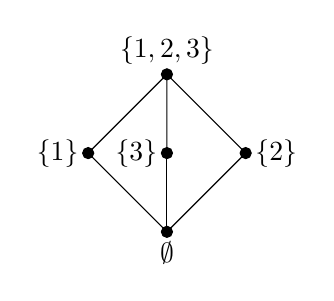
\begin{tikzpicture}
			\filldraw[black] (1,1) circle (2pt) node[anchor=south]{$\{1,2,3\}$};
			\filldraw[black] (0,0) circle (2pt) node[anchor=east]{$\{1\}$};
			\filldraw[black] (2,0) circle (2pt) node[anchor=west]{$\{2\}$};
			\filldraw[black] (1,-1) circle (2pt) node[anchor=north]{$\emptyset$};
			\filldraw[black] (1,0) circle (2pt) node[anchor=east]{$\{3\}$};
			\draw[-,thin] (1,0)--(1,1)--(0,0)--(1,-1)--(2,0)--(1,1);
			\draw[-,thin](1,0)--(1,-1);
		\end{tikzpicture}
	\end{center}
	\item Consideriamo $B=\{\emptyset, \{1\}, \{2\}, \{2,3\},\{1,2,3\} \}$. Si ottiene il reticolo pentagonale:
	\begin{center}
		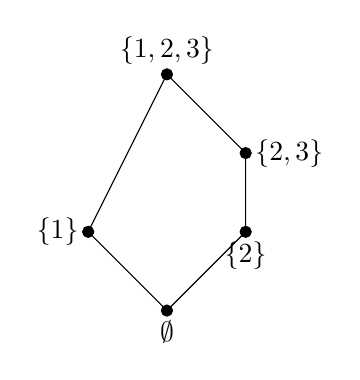
\begin{tikzpicture}
			\filldraw[black] (2,3) circle (2pt)node[anchor=south]{$\{1,2,3\}$};
			\filldraw[black] (3,2) circle (2pt)node[anchor=west]{$\{2,3\}$};
			\filldraw[black] (1,1) circle (2pt)node[anchor=east]{$\{1\}$};
			\filldraw[black] (2,0) circle (2pt) node[anchor=north]{$\emptyset$};
			\filldraw[black] (3,1) circle (2pt)node[anchor=north]{$\{2\}$};
			\draw[-,thin] (2,3)--(1,1)--(2,0)--(3,1)--(3,2)--(2,3);
		\end{tikzpicture}
	\end{center}
\end{enumerate}
\begin{exsbox}
	Dimostrare in modo diretto che gli insiemi totalmente ordinati sono reticoli distributivi.
\end{exsbox}
\paragraph{Svolgimento.} Sia $(S,\leq)$ un insieme totalmente ordinato. Ovviamente, per definizione di relazione d'ordine totale, per ogni parte $\{a,b\}$ di elementi di $S$ esiste un minimo ed un massimo, in quanto vale $a \leq b$ oppure $b \leq a$. Ovvero, posto $a \leq b$:
\begin{align*}
	a \wedge b = inf(\{a,b\}) = a \\
	a \vee b =  sup(\{a,b\}) = b
\end{align*}Si determina cioè una catena. Presi quindi $a,b,c \in S(a \leq b \leq c)$, vale:
\begin{align*}
	a \vee (b \wedge c) =  a \vee b = b \\
	(a \vee b) \wedge (a \vee c) = b \wedge c = b
\end{align*}
E vale:
\begin{align*}
	a \wedge(b \vee c) = a \wedge c  = a\\
	(a \wedge b) \vee (a \wedge c) = a \vee a = a 
\end{align*}
Quindi il reticolo risulta essere distributivo. \hfill \blacksquare
\begin{exsbox}
	Sia $X=\{n \in \mathbb{N} \; | \; 1 \leq n \leq 10\}$. Si considerino i seguenti insiemi di parti di $X$:
	\begin{align*}
		A = \bigl\{\{1,3,5\},\{4,6\}, \{1,7,8\},\{9,10\}\bigr\} \\
		B= \bigl\{\{4\}, \{5,8\},\{1,2,3\},\{6,7,9,10\}\bigr\}
	\end{align*}
Quale tra $A$ e $B$ è una partizione di $X$? Quale non lo è? (giustificare \textit{entrambe} le risposte).
Detta $F$ quella tra $A$ e $B$ che è una partizione di $X$, per ogni $x \in X$ si indichi con $F_{x}$ l'unico elemento di $F$ tale che $x \in F_{x}$. Si consideri in $X$ la relazione binaria $\Sigma$ così definita:
\begin{align*}
	\forall x,y \in X \bigl(x \ \Sigma \ y \iff (x=y \lor |F_{x}| < |F_{y}|)\bigr)
\end{align*}
\begin{enumerate}[label=(\textit{\roman*})]
	\item Si verifichi che $\Sigma$ è una relazione d'ordine in $X$ e si dica se è totale.
	\item Disegnare il diagramma di Hasse di $(X,\Sigma)$
	\item $(X,\Sigma)$ è un reticolo?
	\item Determinare un sottoinsieme di $X$ di ordine 6 tale che $(Y,\Sigma)$ sia un reticolo. $(Y,\Sigma)$ è distributivo? È complementato?
\end{enumerate}
\end{exsbox}
\paragraph{Svolgimento.} Chiaramente $A$ \textit{non} è una partizione di $X$ in quanto risultano essere presenti parti non disgiunte ed elementi di $X$ mancanti. Ad esempio $\{1,3,5\} \cap \{1,7,8\} = \{1\}$ e $\neg(\exists y \in A)(\{2\}\subseteq y)$. L'insieme delle parti $B$ risulta invece essere una partizione per $X$ in quanto ogni elemento di $B$ è disgiunto da qualsiasi altro elemento della partizione e l'unione unaria di $B$ coincide con $X$. Possiamo quindi porre $F=B$.
\begin{enumerate}[label=(\textit{\roman*})]
	\item Dimostriamo che $\Sigma \in OL(X)$:
	\begin{itemize}
		\item Sicuramente $\Sigma$ è riflessiva in quanto per ogni $x \in X$ vale $x \ \Sigma \ x$ dato che $x=x$.
		\item Siano $x,y \in X$ tale che $x \ \Sigma \ y$ e $y \ \Sigma \ x$. Allora o $x=y$, per definizione della relazione $\Sigma$, oppure, da $|F_{x}|< |F_{y}|$ e $|F_{y}|<|F_{y}|$ segue $|F_{x}|=|F_{y}|$. Poiché in $F$ non sono presenti parti equipotenti devono coincidere $F_{x}$ ed $F_{y}$ per avere lo stesso numero di elementi. Quindi $x,y \in F_{x}$. Ma essendo per ipotesi $x \ \Sigma \ y$ e $y \ \Sigma \ x$ e $|F_{x}| \cancel{<} |F_{x}|$ deve essere per forza $x=y$. Quindi $\Sigma$ risulta essere antisimmetrica.
		\item Siano $x,y,z \in X$ tali che $x \ \Sigma \ y$ e $y \ \Sigma \ z$. Allora o è $x=y$ e $y=z$, da cui $x=z$ e quindi $x \ \Sigma \ z$, oppure $|F_{x}| < |F_{y}| < |F_{z}|$ da cui $|F_{x}| < |F_{z}|$ e $x \ \Sigma \ z$. Quindi $\Sigma$ è transitiva e quindi una relazione d'ordine in $X$.
	\end{itemize}
\item Osservando l'insieme $B$ possiamo osservare che $\Sigma$ è determinata dall'ordine stretto tra le cardinalità delle parti di $B$:
\begin{displaymath}
|\{4\}| < |\{5,8\}| <|\{1,2,3\}| < |\{6,7,9,10\}|
\end{displaymath}
Due elementi nello stesso $F_{x}$ sono in relazione $\Sigma$ se e solo se questi coincidono. Quindi due elementi distinti risultano sempre inconfrontabili in uno stesso $F_{x}$. Otteniamo quindi il seguente diagramma di Hasse:
\begin{center}
	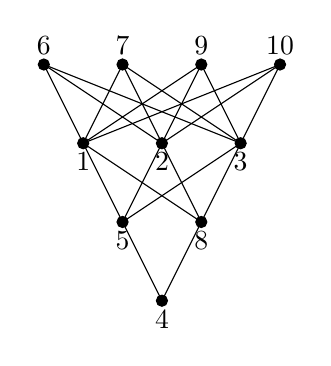
\begin{tikzpicture}
		\filldraw[black] (0,0) circle(2pt) node[anchor=north]{4};
		\filldraw[black] (-0.5,1) circle(2pt) node[anchor=north]{5};
		\filldraw[black] (0.5,1) circle(2pt) node[anchor=north]{8};
		\filldraw[black] (-1,2) circle(2pt) node[anchor=north]{1};
		\filldraw[black] (0,2) circle(2pt) node[anchor=north]{2};
		\filldraw[black] (1,2) circle(2pt) node[anchor=north]{3};
		\filldraw[black] (-1.5,3) circle(2pt) node[anchor=south]{6};
		\filldraw[black] (-0.5,3) circle(2pt) node[anchor=south]{7};
		\filldraw[black] (0.5,3) circle(2pt) node[anchor=south]{9};
		\filldraw[black] (1.5,3) circle(2pt) node[anchor=south]{10};
		\draw[black](0,0)--(-0.5,1);
		\draw[black](0,0)--(0.5,1);
		
		\draw[black](0.5,1)--(-1,2);
		\draw[black](0.5,1)--(0,2);
		\draw[black](0.5,1)--(1,2);
		
		\draw[black](-0.5,1)--(-1,2);
		\draw[black](-0.5,1)--(0,2);
		\draw[black](-0.5,1)--(1,2);
		
		\draw[black](-1,2)--(-1.5,3);
		\draw[black](-1,2)--(-0.5,3);
		\draw[black](-1,2)--(0.5,3);
		\draw[black](-1,2)--(1.5,3);
		
		\draw[black](0,2)--(-1.5,3);
		\draw[black](0,2)--(-0.5,3);
		\draw[black](0,2)--(0.5,3);
		\draw[black](0,2)--(1.5,3);
		
		\draw[black](1,2)--(-1.5,3);
		\draw[black](1,2)--(-0.5,3);
		\draw[black](1,2)--(0.5,3);
		\draw[black](1,2)--(1.5,3);
	\end{tikzpicture}
\end{center}
\item Dato che in un reticolo finito devono esiste minimo e massimo, osservando il fatto che risultano esserci 4 elementi massimali possiamo affermare che $(X,\Sigma)$ non risulta essere un reticolo.
\item Sicuramente la parte $Y=\{4,8,1,2,3,10\}$ risulta formare un reticolo con la relazione $\Sigma$:

\begin{center}
	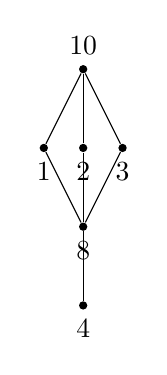
\begin{tikzpicture}
		\node[circle,fill=black,inner sep=0pt,minimum size=3pt,label=below:{4}](4) at (0,0){};
		\node[circle,fill=black,inner sep=0pt,minimum size=3pt,label=below:{8}](8) at (0,1){};
		\node[circle,fill=black,inner sep=0pt,minimum size=3pt,label=below:{1}](1) at (-0.5,2){};
		\node[circle,fill=black,inner sep=0pt,minimum size=3pt,label=below:{2}](2) at (0,2){};
		\node[circle,fill=black,inner sep=0pt,minimum size=3pt,label=below:{3}](3) at (0.5,2){};
		\node[circle,fill=black,inner sep=0pt,minimum size=3pt,label=above:{10}](10) at (0,3){};
		\draw[black,thin](4)--(8);
		\draw[black,thin](8)--(1);
		\draw[black,thin](8)--(2);
		\draw[black,thin](8)--(3);
		\draw[black,thin](1)--(10);
		\draw[black,thin](2)--(10);
		\draw[black,thin](3)--(10);
	\end{tikzpicture}
\end{center}
$(Y,\Sigma)$ non è complementato. Infatti preso l'elemento $3 \in Y$ si vede facilmente che non ha complemento. 
\begin{center}
	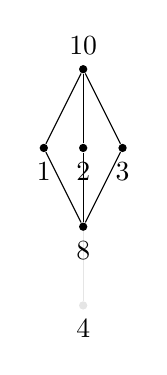
\begin{tikzpicture}
		\node[circle,fill=black,inner sep=0pt,minimum size=3pt,label=below:{4},opacity=0.1](4) at (0,0){};
		\node[circle,fill=black,inner sep=0pt,minimum size=3pt,label=below:{8}](8) at (0,1){};
		\node[circle,fill=black,inner sep=0pt,minimum size=3pt,label=below:{1}](1) at (-0.5,2){};
		\node[circle,fill=black,inner sep=0pt,minimum size=3pt,label=below:{2}](2) at (0,2){};
		\node[circle,fill=black,inner sep=0pt,minimum size=3pt,label=below:{3}](3) at (0.5,2){};
		\node[circle,fill=black,inner sep=0pt,minimum size=3pt,label=above:{10}](10) at (0,3){};
		\draw[black,thin,opacity=0.1](4)--(8);
		\draw[black,thin](8)--(1);
		\draw[black,thin](8)--(2);
		\draw[black,thin](8)--(3);
		\draw[black,thin](1)--(10);
		\draw[black,thin](2)--(10);
		\draw[black,thin](3)--(10);
	\end{tikzpicture}
\end{center}
Applicando infine il Criterio di Birkhoff osserviamo che è possibile individuare un sottoreticolo di $(Y,\Sigma)$ isomorfo al reticolo trirettangolo, quindi $Y$ non è distributivo. \hfill \blacksquare
\end{enumerate} 
\begin{exsbox}
	Sia $A=\{1,2,3\} \times \{1,2,3\}$. Si consideri la relazione $R$ definita su $A$ come segue:
	\begin{displaymath}
		(a,b) \ R \ (c,d) \iff a \leq c \land b \divides d
	\end{displaymath}
	\begin{enumerate}
		\item Dimostrare che $R$ è una relazione d'ordine parziale;
		\item Determinare gli elementi massimali e minimali di $A$. Stabilire se esistono massimo e minimo;
		\item Stabilire se $A$, munito della relazione d'ordine $R$, è un reticolo.
	\end{enumerate}
\end{exsbox}
\paragraph{Svolgimento.} Dimostriamo che $R$ sia una relazione d'ordine:
\begin{enumerate}
	\item Per ogni $(a,b) \in A$ si ha che $a \leq a$ e $b \divides b$, dunque $(a,b) \ R \ (a,b)$.
	\item Supponiamo di avere due coppie $(a,b)$ e $(c,d)$ tali che $(a,b) \ R \ (c,d)$ e $(c,d) \ R \ (a,b)$. Allora deve essere $a \leq c$ e $c \leq a$ da cui $a =c$ e deve essere $b \divides d$ e $d \divides b$, da cui segue $b=d$. Allora $(a,b)=(c,d)$.
	\item Se $a \leq c$ e $b \divides d$ e $c \leq e$ e $d \divides f$, allora $a \leq e$ e $b \divides f$. Quindi $R$ risulta riflessiva, antisimmetrica e transitiva. Quindi è una relazione d'ordine parziale.
\end{enumerate}
Per cercare elementi minimali o massimali ed eventuali massimi e minimi possiamo notare che la coppia $(1,1)$ è in relazione con tutte le coppie $(a,b) \in A$ e risulta quindi un minimo. Al contrario, le coppie $(3,2)$ e $(3,3)$ risultano elementi massimali. 
\begin{center}
	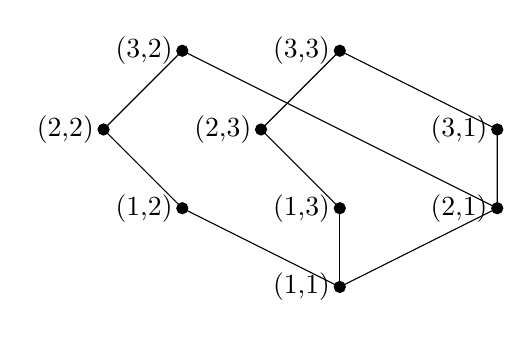
\begin{tikzpicture}
		\filldraw[black] (0,0) circle (2pt) node[anchor=east]{(1,1)};
		\filldraw[black] (-2,1) circle (2pt) node[anchor=east]{(1,2)};
		\filldraw[black] (0,1) circle (2pt) node[anchor=east]{(1,3)};
		\filldraw[black] (2,1) circle (2pt) node[anchor=east]{(2,1)};
		\filldraw[black] (-3,2) circle (2pt) node[anchor=east]{(2,2)};
		\filldraw[black] (-1,2) circle (2pt) node[anchor=east]{(2,3)};
		\filldraw[black] (2,2) circle (2pt) node[anchor=east]{(3,1)};
		\filldraw[black] (-2,3) circle (2pt) node[anchor=east]{(3,2)};
		\filldraw[black] (0,3) circle (2pt) node[anchor=east]{(3,3)};
		\draw[black](0,0)--(-2,1);
		\draw[black](0,0)--(0,1);
		\draw[black](0,0)--(2,1);
		\draw[black](-2,1)--(-3,2);
		\draw[black](-3,2)--(-2,3);
		\draw[black](-1,2)--(0,3);
		\draw[black](0,1)--(-1,2);
		\draw[black](2,1)--(2,2)--(0,3);
		\draw[black](2,1)--(-2,3);
	\end{tikzpicture}
\end{center}
Dato che non esiste estremo superiore per la parte $\{(3,2),(3,3)\}$ possiamo affermare che $(A,R)$ non è un reticolo. \hfill \blacksquare
\begin{exsbox}
	Sull'insieme $A=\{a^{n} \; | \; a,n \in \mathbb{N},a,n \geq 2\} \subseteq \mathbb{N}$ si definisca la relazione $\unlhd$ ponendo:
	\begin{displaymath}
		a^{n} \unlhd b^{m} \iff a \divides b \land n \leq m
	\end{displaymath}
	Si dica se $\unlhd$ è una relazione d'ordine su $A$.
\end{exsbox}
\paragraph{Svolgimento.} Gli elementi di $A$ non sono rappresentati univocamente da una coppia $(a,n)$. Ad esempio $2^{4}=4^{2}$. Si vede allora che la relazione proposta dall'esercizio non è ben definita: infatti da un lato risulterebbe $2^{4} \unlhd 2^{5}$(dato che $2 \divides 2$ e $4 \leq 5$) mentre anche $4^{2} \cancel{\unlhd} 2^{5}$ (dato che $4 \ndivides 2$). \hfill \blacksquare
\begin{exsbox}
	Sull'insieme $A=\mathbb{N} \times \mathbb{N}$ si definisca la relazione $\unlhd$ ponendo, per ogni $(a,b),(c,d) \in A$,
	\begin{displaymath}
		(a,b) \unlhd (c,d) \iff \begin{cases}
			a \leq c \\
			a+d \leq b+c
		\end{cases}
	\end{displaymath}
	\begin{enumerate}
		\item Si provi che $\unlhd$ è una relazione d'ordine e che non è totale;
		\item Osservato che per ogni $(a,b) \in A$ si ha $(a,b) \unlhd (a+1,b)$, si provi che l'insieme ordinato $(A,\unlhd)$ non ha né elementi massimali né minimali.
		\item Posto $x=(0,0)$ e $y=(1,2)$ si provi che $inf_{A}\{x,y\}=(0,1)$.
	\end{enumerate}
\end{exsbox}
\paragraph{Svolgimento.} Si ha:
\begin{enumerate}
	\item Proviamo che $\unlhd$ è una relazione d'ordine su $A$:
	\begin{itemize}
		\item \textit{Riflessività.} Per ogni $(a,b) \in A$ si ha banalmente $a \leq a$ e $a+b \leq b+a$; dunque $(a,b)\unlhd(a,b)$.
		\item \textit{Antisimmetria.} Siano $(a,b),(c,d) \in A$ con $(a,b) \unlhd (c,d)$ e $(c,d) \unlhd (a,b)$; allora:
		\begin{displaymath}
			\begin{array}{ll}
				\begin{cases}
					a \leq c \\
					a+d \leq b+c
				\end{cases}
				&
				\begin{cases}
					c \leq a \\
					c+b \leq d+a
				\end{cases}
			\end{array}
		\end{displaymath}
		da cui segue subito $c=a$ e $d=(c+b)-a=a+b-a=b$.
		\item \textit{Transitività.} Siano $(a,b),(c,d),(e,f) \in A$ con $(a,b) \unlhd (c,d)$ e $(c,d) \unlhd (e,f)$ allora:
		\begin{displaymath}
			\begin{array}{ll}
				\begin{cases}
					a \leq c \\
					a+d \leq b+c
				\end{cases}
				&
				\begin{cases}
					c \leq e \\
					c+f \leq d+e
				\end{cases}
			\end{array}
		\end{displaymath}
		da cui si ricava $a \leq e$ e:
		\begin{align*}
			a+f &= a+d-d+f \\
			&\leq b+c-d+f \\
			&= (c+f)-d+b \\
			&\leq e+d-d+b \\
			&= e+b
		\end{align*}
		Dunque $(a,b) \unlhd (e,f)$. Quindi $(A,\unlhd)$ è un insieme ordinato. L'ordine non è totale perché, ad esempio, $(0,0) \cancel{\unlhd} (1,2)$ e $(1,2) \cancel{\unlhd} (0,0)$.
	\end{itemize}
	\item Sia $(a,b) \in A$. Allora, come si verifica subito dalla definizione $(a,b) \unlhd (a+1,b)$ e $(a,b+1) \unlhd (a,b)$. Questo prova che $(A,\unlhd)$ non ha elementi massimali né minimali.
	\item Sia $u=(a,b) \in A$. Allora $u \unlhd x$ se e solo se $a \leq 0$ e $a+0 \leq b+0$, cioè se e solo se $a=0$; mentre $u \unlhd y$ se e solo se $a \leq 1$ e $a+2 \leq b+1$, ovvero se e solo se $a=0,1$ e $b \geq a+1$. Pertanto l'insieme degli elementi minoranti di $\{x,y\}$ è:
	\begin{displaymath}
		\mathcal{M} = \{(0,b) \in A \; | \; b \geq 1\}
	\end{displaymath}
	Ora, per ogni $b \geq 1$ si ha $(0,b) \unlhd (0,1)$. Ne consegue che $(0,1)$ è il massimo di $\mathcal{M}$ e dunque è l'estremo inferiore di $\{x,y\}$.
	\begin{flushright}
		\blacksquare
	\end{flushright}
\end{enumerate}

\begin{exsbox}
	Sull'insieme $A = \{(x,y) \; | \; x,y \in \mathbb{N} \land x,y \geq 2\}$ si definisca la relazione $\unlhd$ ponendo:
	\begin{displaymath}
		(a,b) \unlhd (c,d) \iff (a \leq c \land b \divides d)
	\end{displaymath}
	\begin{enumerate}
		\item Si provi che $\unlhd$ è una relazione d'ordine su $A$;
		\item Si determini gli eventuali massimo, minimo ed elementi massimali e minimali di $(A,\unlhd)$.
		\item Sia $D=\{(x,y) \in A \; | \; x+y=10\}$ si determinino, se esistono $inf_{A}(D)$ e $sup_{A}(D)$.
	\end{enumerate}
\end{exsbox}

\paragraph{Svolgimento.} Abbiamo:
\begin{enumerate}
	\item Per dimostrare che $\unlhd$ è una relazione d'ordine verifichiamo che soddisfi le proprietà riflessive, antisimmetriche e transitive:
	\begin{itemize}
		\item Per ogni coppia $(a,b)$ deve essere $(a,b) \unlhd (a,b)$, infatti:
		\begin{displaymath}
			(a,b) \unlhd (a,b) \iff (a \leq a \land b \divides b)
		\end{displaymath}
		e $\unlhd$ risulta riflessiva;
		\item Siano $(a,b)$ e $(c,d)$ due coppie tali che $(a,b) \unlhd (c,d)$ e $(c,d) \unlhd (a,b)$. Abbiamo quindi:
		\begin{displaymath}
			(a \leq c \land b \divides d) \land (c \leq a \land d \divides b) \iff (a=c \land b=d) \iff (a,b) = (c,d)
		\end{displaymath}
		per l'antisimmetria della relazione d'ordine usuale in $\mathbb{N}$ e per le proprietà\footnote{Vedi \ref{sez:associati}.} degli elementi associati in $\mathbb{N}$. La relazione $\unlhd$ risulta quindi antisimmetrica.
		\item Siano $(a,b),(c,d),(e,f)$ tre coppie di $A$ tali che $(a,b) \unlhd (c,d) \land (c,d) \unlhd (e,f)$. Abbiamo allora:
		\begin{displaymath}
			(a \leq c \land b \divides d) \land (c \leq e \land d \divides f)
		\end{displaymath}
		Per la transitività della relazione d'ordine usuale abbiamo $a \leq e$. Inoltre, se $b \divides d$ e $d \divides f$ abbiamo:
		\begin{align*}
			\exists k \in \mathbb{N} (d=kb) \land \exists h \in \mathbb{N}(f=hd) \implies f=h(kb)=b(hk) \\
		\end{align*}
		e quindi $b \divides f$. Allora $(a,b) \unlhd (e,f)$ e $\unlhd$ è una relazione d'ordine.
	\end{itemize}
	\item Per ogni $(a,b) \in A$ osserviamo che $(a,b) \unlhd (a+1,b)$ quindi non ci sono elementi massimali (non esiste un elemento $(\overline{a},\overline{b})$ di $A$ tale che per ogni $(a,b) \in A$ si abbia $(a,b) \unlhd (\overline{a},\overline{b})$) e dunque nemmeno massimi in $(A,\unlhd)$. Per quanto riguarda invece gli elementi minimali, consideriamo le coppie del tipo $(2,p)$ con $p$ numero primo positivo: se $(a,b) \unlhd (2,p)$ allora $a \leq 2$ e $b \divides p$, da cui, poiché $a,b \geq 2$, si ha $(a,b)=(2,p)$. Quindi $(2,p)$ è un elemento minimale di $(A,\unlhd)$. Poiché esistono più elementi minimali allora non esiste il minimo.
	\item Chiaramente $D=\{(2,8),(3,7),(4,6),(5,5),(6,4),(7,3),(8,2)\}$. Sia $(a,b) \in A$ un elemento minorante per $D$ allora in particolare $(a,b) \unlhd (2,8)$, dunque $a=2$ e $b \divides 8$, ma anche $(a,b) \unlhd (3,7)$ da cui $b \divides 7$. Poiché $b \geq 2$, questo non è possibile. Pertanto non esistono minoranti, quindi nemmeno estremo inferiore di $D$. Sia ora $(a,b) \in A$ un maggiorante di $D$. Allora $x \leq a $ e $y \divides b$ per ogni $2 \leq x,y \in \mathbb{N}$ con $x+y=10$. Poiché il minimo comune multiplo di 2, 3, 4, 5, 6, 7, 8 risulta essere 840, si conclude che $8 \leq a$ e $840 \divides b$. L'insieme dei maggioranti per $D$ è dunque $\{(a,b) \in A \; | \; 8 \leq a, 840 \divides b\}$. Tale insieme ha un evidente minimo in $(A,\unlhd)$ che è $(8,840)$ ed è l'estremo superiore di $D$. \hfill \blacksquare
\end{enumerate}
\begin{exsbox}
	Sull'insieme $\mathcal{P}(\mathbb{N})$ si definisca la relazione $\unlhd$ definita da:
	\begin{displaymath}
		\forall X,Y \in \mathcal{P}(\mathbb{N}) \bigl(X \unlhd Y \iff X \subseteq Y \land Y \setminus X \text{ è finito}\bigr)
	\end{displaymath}
	\begin{enumerate}
		\item Si provi che $\unlhd$ è una relazione d'ordine su $\mathcal{P}(\mathbb{N})$ e si dica se è totale;
		\item Si dica se l'insieme ordinato $(\mathcal{P}(\mathbb{N}),\unlhd)$ ha elementi minimali e/o minimi;
	\end{enumerate}
\end{exsbox}
\paragraph{Svolgimento.} Abbiamo:
\begin{enumerate}
	\item Proviamo che $\unlhd$ è una relazione d'ordine su $\mathcal{P}(\mathbb{N})$:
	\begin{itemize}
		\item \textit{Riflessività.} Sia $X \in \mathcal{P}(\mathbb{N})$ allora $X \subseteq X$ e $X \setminus X = \emptyset$, quindi $X \unlhd X$;
		\item \textit{Antisimmetria.} Siano $X,Y \in \mathcal{P}(\mathbb{N})$ con $X \unlhd Y$ e $Y \unlhd X$; allora in particolare $X \subseteq Y$ e $Y \subseteq X$, quindi $X=Y$;
		\item \textit{Transitività.} Siano $X,Y,Z \in \mathcal{P}(\mathbb{N})$ con $X \unlhd Y$ e $Y \unlhd Z$. Allora in particolare $X \subseteq Y$ e $Y \subseteq Z$, dunque $X \subseteq Z$. Inoltre, poiché $X$ è contenuto in $Y$, $Y=X \cup (Y \setminus X)$ e analogamente $Z = Y \cup (Z \setminus Y)$ con $Y \setminus X$ e $Z \setminus X$ finiti. Quindi:
		\begin{displaymath}
			Z = Y \cup (Z \setminus Y) = Z = X \cup (Y \setminus X) \cup (Z \setminus Y)
		\end{displaymath}
		dunque $Z \setminus X \subseteq (Y \setminus X) \cup (Z \setminus Y)$ è finito e $X \unlhd Z$. Pertanto $(\mathcal{P}(\mathbb{N}),\unlhd)$ è un insieme ordinato. Chiaramente non è totale, ad esempio $\{1\} \cancel{\unlhd} \{2\}$ e $\{2\} \cancel{\unlhd} \{1\}$.
	\end{itemize}
	\item $\emptyset$ è un elemento minimale dell'insieme ordinato ma non è minimo. Infatti se $X$ è un sottoinsieme infinito di $\mathbb{N}$ allora $\varnothing \cancel{\unlhd} X$. Non vi sono altri elementi minimali, infatti se $0 \neq X \subseteq \mathbb{N}$ e $a \in X$ allora $X \setminus \{a\} \unlhd X$. \hfill \blacksquare
\end{enumerate}

\begin{exsbox}
	Sia $S=\{a,b,c,d,e,f,g\}$ dove $a=\varnothing$, $b=\{1\}$, $c=\{2,3\}$, $d=\{4\}$, $e= \mathbb{N}\setminus 2\mathbb{N}$, $f=\{2^{n}/n \in \mathbb{N}\}$, $g=\mathbb{N}$.
	\begin{enumerate}
		\item Disegnare il diagramma di Hasse di $(S,\subseteq)$;
		\item Decidere se $(S,\subseteq)$ sia un reticolo;
		\item Verificare se $(S,\subseteq)$ è distributivo, complementato o booleano;
		\item $(S,\subseteq)$ è un sottoreticolo di $(\mathcal{P}(\mathbb{N}),\subseteq)$?
		\item Determinare, se esiste, un $h \in \mathcal{P}(\mathbb{N})$ tale che $(S \cup \{h\},\subseteq)$ sia un reticolo booleano.
	\end{enumerate}
\end{exsbox}

\paragraph{Svolgimento.} Svolgiamo punto per punto:
\begin{enumerate}
	\item L'idea è quella di partire dal basso, ovvero dall'insieme che sicuramente è incluso in tutti gli altri elementi di $S$, ossia l'elemento $a= \varnothing$. Successivamente notiamo che $b$, $c$ e $d$ sono tre elementi non confrontabili tra di loro che sicuramente includono $a$. Questi tre elementi faranno quindi parti del ``livello'' successivo. L'elemento $d$, essendo il singleton di 4 sicuramente è una parte di $f$ in quanto $4=2^{n} \in f$ mentre $b$, essendo il singleton di 1, ovvero un numero dispari, sicuramente è una parte di $f$ ma anche di $f$ in quanto $1=2^{0} \in f$. Si ottiene così un secondo livello dato dagli elementi $e$ ed $f$ che sono infine parti di $\mathbb{N}=g$. Il diagramma di Hasse che si ottiene è il seguente:
	\begin{center}
		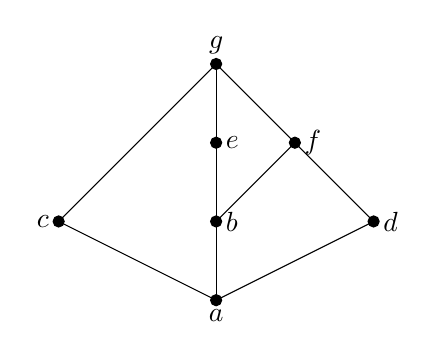
\begin{tikzpicture}
			\filldraw[black](1,0)circle(2pt)node[below]{$a$};
			\filldraw[black](-1,1)circle(2pt)node[left]{$c$};
			\filldraw[black](1,1)circle(2pt)node[right]{$b$};
			\filldraw[black](3,1)circle(2pt)node[right]{$d$};
			\filldraw[black](1,2)circle(2pt)node[right]{$e$};
			\filldraw[black](2,2)circle(2pt)node[right]{$f$};
			\filldraw[black](1,3)circle(2pt)node[above]{$g$};
			\draw[-](1,0)--(-1,1);
			\draw[-](1,0)--(1,1);
			\draw[-](1,0)--(3,1);
			\draw[-](1,1)--(1,2);
			\draw[-](3,1)--(2,2);
			\draw[-](2,2)--(1,3);
			\draw[-](-1,1)--(1,3);
			\draw[-](1,2)--(1,3);
			\draw[-](1,1)--(2,2);
		\end{tikzpicture}
	\end{center}
	\item Per definizione di reticolo deve essere:
	\begin{displaymath}
		\forall x,y \in S \bigl( \exists inf_{\subseteq}\{x,y\} \land \exists sup_{\subseteq} \{x,y\}\bigr)
	\end{displaymath}
	Poiché $\forall x,y \in S$ sono equivalenti le formule $x \subseteq y$, $x = min \{x,y\}$ e $inf \{a,b\}$ basterà confrontare tutte le coppie non confrontabili e stabilire se per queste esistono gli estremi inferiori e superiori. Tali coppie sono:
	\begin{displaymath}
		\begin{array}{llll}
			\{c,b\}, & \{c,d\}, & \{b,d\} & \{e,f\}
		\end{array}
	\end{displaymath}
	e si ha: \begin{displaymath}
		\begin{array}{llll}
			\begin{cases}
				inf_{\subseteq}\{c,b\}=a\\
				sup_{\subseteq}\{c,b\}=g
			\end{cases}
			& \begin{cases}
				inf_{\subseteq}\{c,d\}=a\\
				sup_{\subseteq}\{c,d\}=g
			\end{cases}
			& \begin{cases}
				inf_{\subseteq}\{b,d\}=a\\
				sup_{\subseteq}\{b,d\}=f
			\end{cases}
			& \begin{cases}
				inf_{\subseteq}\{e,f\}=b\\
				sup_{\subseteq}\{e,f\}=g
			\end{cases}
		\end{array}
	\end{displaymath}
	Quindi $(S,\subseteq)$ è un reticolo.
	\item Per il Criterio di Birkhoff $(S,\subseteq)$ non è distributivo se qualche suo sottoreticolo è isomorfo al reticolo pentagonale oppure al reticolo trirettangolo. Se osserviamo il seguente sottoreticolo:
	\begin{center}
		\begin{tikzpicture}
			\filldraw[black](1,0)circle(2pt)node[below]{$a$};
			\filldraw[black](-1,1)circle(2pt)node[left]{$c$};
			\filldraw[black](1,1)circle(2pt)node[right]{$b$};
			\filldraw[black](3,1)circle(2pt)node[right]{$d$};
			%\filldraw[black](1,2)circle(2pt)node[right]{$e$};
			%\filldraw[black](2,2)circle(2pt)node[right]{$f$};
			\filldraw[black](1,3)circle(2pt)node[above]{$g$};
			\draw[-](1,0)--(-1,1);
			\draw[-](1,0)--(1,1);
			\draw[-](1,0)--(3,1);
			%\draw[-](1,1)--(1,2);
			%\draw[-](3,1)--(2,2);
			%\draw[-](2,2)--(1,3);
			\draw[-](-1,1)--(1,3);
			%\draw[-](1,2)--(1,3);
			%\draw[-](1,1)--(2,2);
			\draw[-](1,1)--(1,3);
			\draw[-](3,1)--(1,3);
		\end{tikzpicture}
	\end{center}
	Si vede che è isomorfo al reticolo trirettangolo. Concludiamo così che $(S,\subseteq)$ non è distributivo.
	
	Per definizione di reticolo complementato, $(S,\subseteq)$ deve essere un reticolo limitato (ovvero devono esistere minimo e massimo) ed ogni elemento del reticolo deve ammettere almeno un complemento: ovvero per ogni $x \in S$ deve esistere un $y \in S$ tale che
	\begin{displaymath}
		\bigl(x \wedge y = min(S,\subseteq) = a \bigr) \land \bigl(	x \vee y = max(S,\subseteq)= g\bigr)
	\end{displaymath}
	Chiaramente $(S,\subseteq)$ è limitato e la richiesta ha senso. Se prendiamo ad esempio $g=\mathbb{N}$ e $a=\varnothing$ sono l'uno il complemento dell'altro. Presi quindi $x \in S$ tale che $x \neq g,a,c$ allora:
	\begin{displaymath}
		\begin{cases}
			sup_{\subseteq} \{c,x\} = g = \mathbb{N}\\
			inf_{\subseteq}\{c,x\}= a = \varnothing
		\end{cases}
	\end{displaymath}
	Quindi ogni $x \in S$ diverso da $a,c,g$ è complementato da $c$ (non è l'unico). In particolare $c$ ha $x$ come complemento. Quindi $S$ è complementato. Per definizione di reticolo booleano, $(S,\subseteq)$ deve essere sia distributivo che complementato. Poiché $S$ non è distributivo allora non è booleano.
	\item Per essere un sottoreticolo di $(\mathcal{P}(\mathbb{N}),\subseteq)$ $S$ deve essere stabile secondo le operazioni reticolari del reticolo delle parti di $\mathbb{N}$ ovvero $\cup$ e $\cap$. Notiamo però che:
	\begin{displaymath}
		b \cup c = \{1\} \cup \{2,3\} = \{1,2,3\} \notin S
	\end{displaymath}
	Quindi $S$ non è stabile e di conseguenza non risulta un sottoreticolo. Questa verifica può essere fatta anche osservando il diagramma di Hasse del reticolo $S$. Poiché le operazioni reticolari $\cap$ e $\cup$ mappano ogni coppia del reticolo rispettivamente nel loro estremo inferiore ed estremo inferiore, se si osservano i punti $c$ ed $e$ si ha: $$\{2\} = c \cap e  \neq inf_{\subseteq} \{c,e\} = \varnothing $$
	\item  Il problema del reticolo $S$ era la distributività. Infatti si era dimostrato al punto 3 che il reticolo $S$ non è distributivo in quanto il sottoreticolo $(\{a,c,b,d,g\},\subseteq)$ è isomorfo al reticolo trirettangolo. Essendo il reticolo trirettangolo uno dei più piccoli tra i reticoli non distributivi, aggiungendo un elemento ad $S$ nulla cambierebbe in quanto resterebbe sempre invariato il sottoreticolo $(\{a,c,b,d,g\},\subseteq)$.  \hfill \blacksquare
\end{enumerate}
\begin{exsbox}
	Disegnare un diagramma di Hasse dell'insieme $\{n \in \mathbb{N} / n <10\}$ ordinato per divisibilità in $\mathbb{N}$ e decidere se questo insieme ordinato è un reticolo.
\end{exsbox}
\begin{exsbox}
	Per ogni $n \in \{8,12,18,30,31,2^{10}\}$ disegnare un diagramma di Hasse dell'insieme $D_{n}$ dei divisori (in $(\mathbb{N},\cdot)$) di $n$, ordinato per divisibilità in $\mathbb{N}$, e decidere se $(D_{n},\divides)$ è o non è un reticolo. Trovare tra questi insiemi ordinati, quali sono isomorfi tra loro.
\end{exsbox}
\begin{exsbox}
	Esiste in $\mathcal{P}(\mathbb{N})$ una parte infinita che sia totalmente ordinata per inclusione (cioè dall'ordinamento indotto dall'inclusione in $\mathcal{P}(\mathbb{N})$)?
\end{exsbox}
\begin{exsbox}
	In ciascuno dei seguenti insiemi, ordinati dalla relazione di inclusione, determinare gli eventuali minimali, massimali, minimo, massimo:
	\begin{enumerate}
		\item $\mathcal{P}(\mathbb{Z})$
		\item $\mathcal{P}_{fin}(\mathbb{Z})$ (l'insieme delle parti finite di $\mathbb{Z}$)
		\item $\mathcal{P}(\mathbb{Z})\setminus \mathcal{P}_{fin}(\mathbb{Z})$ (l'insieme delle parti infinite di $\mathbb{Z}$)
		\item $\mathcal{P}(\mathbb{Z}) \setminus \mathcal{P}(\mathbb{N})$
	\end{enumerate}
\end{exsbox}
\begin{exsbox}
	La relazione binaria $\tau$ definita in $\mathbb{N}$ ponendo, per ogni $a,b \in \mathbb{N}$, $a \tau b$ se e solo se $b−a \in \mathbb{N} \setminus\{1\}$ è d'ordine?
\end{exsbox}

\begin{exsbox}
	Sia $X=\{a,b,c,d,e,f,g,h\}$ in modo che valga $|X|=8$. Verificare che la relazione binaria $\rho$ in $X$ di grafico:
	\begin{displaymath}
		\left\lbrace
		\begin{array}{lllll}
			(a,b), & (a,c), & (a,d), & (a,e), & (a,f), \\
			(a,g), & (a,h), & (b,d), & (b,e), & (b,f), \\
			(b,g), & (b,h), & (c,d), & (c,e), & (c,f), \\
			(c,g), & (c,h), & (d,e), & (d,f), & (d,g), \\
			(d,h), & (e,f), & (g,f)
		\end{array}
		\right\rbrace
	\end{displaymath}
	è un ordinamento in $X$ e disegnarne il diagramma di Hasse. Rispetto a questo ordinamento si indichino gli eventuali minimo, massimo, elementi minimali, elementi massimali in $X$. Se esistono, si calcolino $sup\{b,c,h\}$, $inf\{b,c,h\}$, $sup\{b,e,h\}$, $inf\{b,e,h\}$. Quali elementi di $X$ sono confrontabili con ogni altro elemento di $X$? Infine, si stabilisca se $X$ ordinato da $\rho$ è un insieme totalmente ordinato, un reticolo, un reticolo completo, un reticolo distributivo, un'algebra di Boole.
\end{exsbox}
\begin{exsbox}
	Trovare un isomorfismo di reticoli dall'insieme delle parti di $\{0,1\}$ all'insieme delle parti di $\{3,4\}$, ordinati per inclusione.
\end{exsbox}

\begin{exsbox}
	Stabilire per quali interi $n$ nell'insieme $\{2,14,18,27,30\}$ il reticolo dei numeri naturali divisori di $n$ è complementato.
\end{exsbox}

\begin{exsbox}
	Trovare, tra i sottoinsiemi di $\mathcal{P}(\mathbb{N})$, ordinati per inclusione:
	\begin{enumerate}
		\item un sottoinsieme di cardinalità 5 che non sia un reticolo;
		\item un sottoinsieme di cardinalità 5 che sia un reticolo trirettangolo;
		\item un sottoinsieme di cardinalità 5 che sia un reticolo pentagonale.
	\end{enumerate}
\end{exsbox}
\begin{exsbox}
	Ogni insieme delle parti, ordinato mediante l’inclusione,
	è un reticolo. Infatti, dimostrare che dati $A, B \subseteq Z$, $inf(A, B) = A \cap B$, e $sup(A, B) = A \cup B$.
\end{exsbox}